%% IEEE Access manuscript -- GENERATED FILE, DO NOT EDIT.
%% Produced from paper/paper.md by paper/scripts/build_tex.py.
%% Edit the Markdown and rebuild; hand edits here are lost on the next build.
\documentclass{ieeeaccess}
\usepackage{cite}
\usepackage{amsmath,amssymb,amsfonts}
\usepackage{algorithmic}
\usepackage{graphicx}
\usepackage{textcomp}
\usepackage{booktabs}
\usepackage{multirow}
\usepackage{tabularx}
\usepackage{listings}
\usepackage{microtype}
\usepackage{url}

%% Typewriter face. The class's default is Courier, which is wide, light and
%% sits badly beside Times and Formata. Inconsolata is narrower and darker,
%% which also shortens the long file paths this manuscript quotes inline.
\IfFileExists{inconsolata.sty}{\usepackage[scaled=0.95,varqu]{inconsolata}}{%
  \IfFileExists{beramono.sty}{\usepackage[scaled=0.82]{beramono}}{}}

%% Wide content control. The text block is 177.53mm and a column 85.29mm, so
%% long tokens and wide tables overflow silently unless told how to break.
\lstset{
  basicstyle=\ttfamily\scriptsize,
  breaklines=true,
  breakatwhitespace=false,
  postbreak=\mbox{$\hookrightarrow$\space},   % no colour: the class does not
                                              % define xcolor's named colours
  columns=fullflexible,
  keepspaces=true,
  showstringspaces=false,
  frame=none,
  aboveskip=6pt,
  belowskip=6pt,
}
%% Float placement. Every table and figure here is full-width, and a
%% double-column float can only be set at the top of a page. With LaTeX's
%% defaults -- at most two per page top, filling at most 0.7 of it, and a
%% float page declared as soon as the queue fills 0.5 of one -- the queue
%% drains into pages that are nothing but floats: one page of this manuscript
%% carried four floats and no text at all, several pages after the text that
%% introduces them. Raising the per-page allowance and the fraction a float
%% page must reach lets the queue drain onto the tops of text pages instead.
\setcounter{topnumber}{3}
\setcounter{dbltopnumber}{3}
\setcounter{totalnumber}{4}
\renewcommand{\topfraction}{0.92}
\renewcommand{\dbltopfraction}{0.92}
\renewcommand{\textfraction}{0.08}
\renewcommand{\floatpagefraction}{0.90}
\renewcommand{\dblfloatpagefraction}{0.95}

\Urlmuskip=0mu plus 0.15mu       % enough give to break a long URL, not
                                 % enough to gap it visibly: at plus 1mu
                                 % an 85 mm column rendered the repo URL
                                 % as https : / / github . com / ...
\def\UrlBreaks{\do\/\do-\do.\do_\do:}
\usepackage[colorlinks=true,linkcolor=blue,citecolor=blue,
            urlcolor=blue]{hyperref}
\hypersetup{pdftitle={Auditing Provenance Confounding in Image Authenticity Classification: A Counterfeit-Medicine Case Study},pdfauthor={Sophie Zhu},
            pdfsubject={IEEE Access submission},
            pdfkeywords={Data leakage, dataset bias, domain generalization, external validation, hidden stratification, image classification, provenance confounding, shortcut learning}}
\def\BibTeX{{\rm B\kern-.05em{\sc i\kern-.025em b}\kern-.08em
    T\kern-.1667em\lower.7ex\hbox{E}\kern-.125emX}}

\begin{document}

%% The ieeeaccess class defaults its page footer to VOLUME 11, 2023. Set the
%% submission volume and year so the footer is not stale; IEEE production
%% replaces these along with \history and \doi below.
\vol{14}
\year{2026}

\history{Date of publication xxxx 00, 0000, date of current version
         xxxx 00, 0000.}
\doi{10.1109/ACCESS.2026.DOI}

\title{Auditing Provenance Confounding in Image Authenticity Classification: A Counterfeit-Medicine Case Study}

\author{\uppercase{Sophie Zhu}\authorrefmark{1}}

\address[1]{Mira Costa High School, Manhattan Beach, CA 90266 USA
            (e-mail: sophiezhu2028@gmail.com; ORCID: 0009-0004-2403-910X)}

\tfootnote{This work received no specific grant from any funding agency in the
public, commercial, or not-for-profit sectors.}

\corresp{Corresponding author: Sophie Zhu (e-mail: sophiezhu2028@gmail.com).}

\begin{abstract}
In image authenticity datasets, the inauthentic class is typically scarcer and obtained via alternative routes (e.g., screen-captured, scraped, or generated). Consequently, the label predicts the acquisition process, an association inherited by every data partition. We call this {\bfseries class-conditional provenance confounding} and formalize and operationalize a pre-training {\bfseries provenance audit} for it: fit the classifier the study intends to use to acquisition metadata alone, on the study's own leakage-free partition, reading attributes the object cannot influence separately from mixed proxies. The audit is deliberately simple; a counterfeit-medicine case study shows its value. On a public dataset it returns {\bfseries 1.000}: every counterfeit-labeled file is a PNG screen capture and every authentic-labeled file a JPEG across all 510 images, so three header fields reproduce the labels, and in-distribution accuracy cannot separate packaging from provenance recognition. Two split designs differ by at most 6.8 points and near-duplicate leakage moves accuracy by 0.3. The model reaching 97.4\% authentic-class accuracy on its own test partition recovers 6.0\% of 150 independently sourced authentic photographs. On a balanced external set of 46 regulator-confirmed falsified products against 46 authentic-labeled photographs, balanced accuracy runs 0.478 to 0.652 and only one model excludes chance. An exploratory normalization removes the audited statistics and leaves both corrected backbones depending on the outer region of the frame: removing one provenance signal exposed another. A screen of six further archives shows that the audit discriminates across domains; how often the confound occurs is not established.
\end{abstract}

\begin{keywords}
Data leakage, dataset bias, domain generalization, external validation, hidden stratification, image classification, provenance confounding, shortcut learning.
\end{keywords}

\titlepgskip=-15pt

\maketitle

\section{Introduction}

Substandard and falsified medical products are a persistent global health problem, concentrated in low- and middle-income countries and in unregulated online supply chains \cite{ref1}, \cite{ref2}. Because much falsified product is visually imperfect --- misprinted cartons, wrong color separations, missing batch information --- image-based screening from a consumer smartphone is an attractive triage tool, and a body of work has applied convolutional networks to photographs of medicine packaging and reported high binary accuracy \cite{ref3}, \cite{ref26,ref27,ref28}, alongside a larger literature on pharmaceutical {\itshape identification} rather than {\itshape authentication} \cite{ref4}, \cite{ref5}.

This literature's methodology motivates our approach. There is no shared benchmark for pharmaceutical authentication: each study identified through our targeted literature search built or adopted its own image set, and we did not identify any that reports a check for confounds between acquisition and label (Section II-A). Each reported figure therefore rests on the construction of a single ad hoc collection, and that construction is not examined in the paper reporting it.

{\bfseries The gap this exposes is procedural rather than architectural.} Methods for diagnosing a confounded classifier exist, but they act after the fact, requiring the images and a trained model \cite{ref31}. Missing is a pre-training check, run solely on the files, to establish whether the intended task is separable from data acquisition. This paper formalizes and operationalizes one --- a pre-training {\bfseries provenance audit} that fits the intended classifier to acquisition metadata under the study's own leakage-free split and reports the number --- and demonstrates it through a counterfeit-medicine case study. The audit's ingredients are ordinary, and we do not present it as a new statistical technique; what we specify is when it runs, on which partition, on which variables, and how its score is read.

{\bfseries The central result is easily stated.} On the public counterfeit-medicine dataset audited here, {\bfseries all 510 labels are predictable from container format alone}: every counterfeit-labeled file is a PNG screen capture and every authentic-labeled file a JPEG photograph. High internal classifier performance on this dataset therefore cannot be interpreted as evidence of object-level authentication. Everything else in the paper follows from that result: how to detect it before training, what it costs on independent data, and what happens when it is removed.

\subsection{Asymmetric class sourcing, and what it does to a label}

This asymmetric class availability is not peculiar to pharmaceuticals. In a two-class image dataset asking {\itshape is this genuine?}, authentic examples are typically abundant while the other class is scarce: verified counterfeit stock is hard to obtain for research and often restricted, and forged documents are ordinarily held as evidence. A researcher needing a negative class therefore obtains it {\itshape by some other means than the one that produced the positive class}: screen-capturing regulator bulletins, scraping a different corpus, editing authentic images, or generating examples with a model.

Each such substitution can introduce a systematic difference between the classes unrelated to the property being labeled, because acquisition method influences file format, encoded size, resolution, noise floor, compression signature, color rendering and often backdrop. We call this {\bfseries class-conditional provenance confounding} and identify asymmetric class availability as one mechanism by which it can arise --- a mechanism that is predictable from how a dataset was assembled, which is what makes it auditable in advance.

Let $Y$ be the label and $X$ the image content on which a correct decision would rest. Let $A$ represent file acquisition variables, divided into two types:

\begin{itemize}
\item $A_{\mathrm{pure}}$, attributes fixed by how the file was produced and stored, which the depicted object cannot influence: container format, encoder and its settings, filename pattern, embedded capture timestamps.
\item $A_{\mathrm{mix}}$, attributes jointly determined by acquisition and by content: encoded size, stored dimensions, aspect ratio, and pixel statistics such as mean brightness.
\end{itemize}

The difficulty is not that $A$ exists but that the assembly procedure makes it informative about the label,

\begin{equation*}
I(Y; A) > 0
\end{equation*}


The extreme case, and the one this dataset presents, is

\begin{equation*}
H(Y \mid A_{\mathrm{pure}}) = 0
\end{equation*}


--- the label a deterministic function of variables that carry no information about the object at all. Here container format alone leaves no residual entropy: every counterfeit-labeled file is a PNG and every authentic-labeled file a JPEG, across all 510 images. A {\bfseries provenance audit} measures how close a dataset sits to that extreme by fitting a classifier to $A$ alone and reporting its held-out accuracy, which is, up to sampling error, a lower bound on how well acquisition can predict the label. A high score on $A_{\mathrm{pure}}$ is close to decisive, because storage format is never a property of the photographed object. A high score on $A_{\mathrm{mix}}$ is a reason to investigate, since the separation it detects may belong to the objects rather than to how they were acquired.

\begin{figure*}[!t]
\centerline{
\includegraphics[width=\textwidth]{figures/fig15_mechanism.pdf}}
\caption{The mechanism, and where it is detectable. The boxes are general and carry no numbers; the gray line beneath each is this paper's measurement of that step on the case-study dataset. The audit of Section IV-A reads the third box, which is reachable from a file listing before any model exists.}
\label{fig:1}
\end{figure*}


The condition is damaging because it is {\bfseries the easiest thing in the data to learn}, low-level global statistics being easier to extract than the semantics of a printed carton, and a shortcut-seeking optimizer \cite{ref6} finds them first. It is {\bfseries invisible in-distribution}, because a held-out partition inherits it in the same proportion. And it is {\bfseries silent in the reporting record}, since acquisition method is rarely documented.

The same scarcity is plausible in other authenticity tasks --- counterfeit consumer goods, generated media, forensic document and signature forgery --- wherever an abundant authentic class is paired with an inauthentic one that must be manufactured, seized or harvested separately. We read the case study as an instance of how such datasets can come to be assembled, while being clear that the direct evidence for the mechanism rests on it.

{\bfseries Two independent observations support that reading without establishing its generality.} Running the audit of Section III-E on seven public archives across four application areas, we find the same total confound --- container format alone reproducing the label --- arising in a {\bfseries generated-image} dataset built by different people for a different task, while a signature corpus whose two classes were written on one paper and digitized by one procedure scores at chance on the same axis (Section S-I-W). Independently, Grommelt {\itshape et al.} \cite{ref30} report the mechanism in generated-image detection from the other direction: real images are harvested as lossy JPEGs at modest resolution while generated images are written as lossless PNGs at native size, which on GenImage makes format, compression and size predictive of the label, partly reduces detectors to JPEG detectors, and shifts cross-generator performance by more than 11 points once those factors are equalized.

We separate three levels of evidence and hold to them throughout. {\bfseries Demonstrated}: the case-study dataset is completely provenance-confounded (Section IV-A). {\bfseries Supported}: the mechanism arises outside this dataset and application area, on the two observations just given. {\bfseries Not established}: how frequently it occurs; the seven archives were chosen for accessibility and have no sampling frame, so they show that the audit discriminates across domains and cannot estimate a rate. Table~\ref{tab:6} records every claim against these three levels, and Section V-B states what would count against the mechanism.

\subsection{Contributions and scope}

We evaluated how much reported accuracy survives methodological correction using the Kaggle {\itshape Fake vs Real Medicine} set (661 images), a publicly downloadable collection with no data card and no stated acquisition protocol, typical of what this area works with. Under a protocol fixed in advance, the corrections were identical models under a naive and a near-duplicate-grouped split, four model families from a 97-parameter linear baseline to a 4-million-parameter pretrained backbone, and an external source verified independent rather than assumed so.

The result was not the one the design anticipated. Correcting the split changed in-distribution accuracy by at most 6.8 points; external validation changed the picture. On 150 authentic photographs from an independent source, two of four models classified {\itshape zero} correctly and the model with the highest in-distribution accuracy nine. Looking for an explanation led to the dataset itself and to the result above: its two classes were not merely photographed differently but {\itshape acquired} differently (\texttt{Screenshot*.png} against \texttt{images*.jpg}), and any model, including a 97-parameter linear classifier on a color histogram, has unobstructed access to that difference.

The contributions of this paper are as follows, in descending order of weight.

\begin{itemize}
\item {\bfseries A pre-training provenance audit, formalized and operationalized} (Section III-E). It fits the classifier a study intends to use to acquisition metadata alone, needs no external data, annotation, training run or pixel decoding, and returns {\bfseries 1.000} here from header fields alone. We specify the partition it runs on, the division of variables into those the object cannot influence and those that mix acquisition with content, and how the score is read: a high score establishes that a provenance shortcut is {\itshape available}, not that any model took it. We also report where it fails --- a publisher who normalized an archive before release erased the traces it reads, so that archive scores 0.717 while being confounded at least as severely --- and where it false-alarms (Section IV-A).
\item {\bfseries A case-study finding: the dataset carries a deterministic class--acquisition confound that invalidates in-distribution performance as evidence of authentication ability.} The dataset's listing does not disclose it and no study located by our search reports it; the archive also ships a degenerate split whose training folder is a superset of both others (Sections III-A, IV-A).
\item {\bfseries Evidence that external testing exposes the failure and the leakage correction this literature emphasizes does not.} Re-partitioning at the near-duplicate-cluster level moves accuracy by at most 6.8 points, and a controlled estimate that holds the test set fixed puts the leakage effect at 0.3 points [$-$1.9, +2.4]. On an independent balanced set of 46 regulator-confirmed counterfeits against 46 authentic-labeled photographs, with file-level encoding standardized across the classes and scored once against frozen checkpoints, the four models return balanced accuracies of 0.478, 0.478, 0.543 and 0.652, only the last excluding chance, and the 97-parameter baseline is exposed as a degenerate all-counterfeit classifier that an authentic-only evaluation could not have distinguished from a working one. Under a capture-condition shift the same models recover as little as 6.0\% of plainly authentic photographs (Sections IV-B--IV-D).
\item {\bfseries An exploratory result: removing the acquisition statistics the audit names does not remove every provenance shortcut.} A label-free normalization recovers most of the lost external specificity for two of three models, and region substitution then shows both corrected backbones depending on the outer region of the frame rather than on the packaging at its center (Section IV-E). We do not offer the normalization for use; its role is to show that a correction is itself dataset construction and is owed the same audit.
\end{itemize}

Three things this study does not establish are stated with equal care. It does not estimate how often provenance confounding occurs --- the seven-archive screen of Section IV-A has no sampling frame. It does not measure two-class performance under acquisition shift: the balanced set holds both classes but standardizes file-level acquisition, and the acquisition-shift experiment varies capture but holds one class (Section V-D). And it does not show that any model here can authenticate medicine in the field. We propose no new architecture; no statistically significant difference was detected between the 97-parameter linear model and the 4-million-parameter pretrained network on the internal test partition.

\section{Related Work}

\subsection{Pharmaceutical image authentication}

Image classification has been applied to pharmaceutical products for both {\itshape identification} (which drug is this?) and {\itshape authentication} (is this drug genuine?). Ramos, Samonte and Manlises \cite{ref3} proposed a convolutional neural network authentication system directly comparable in task framing to this work; adjacent identification work addresses look-alike medication errors across 250 blister-packaged drug types \cite{ref4} and pill-image retrieval \cite{ref5}. That literature establishes that packaging imagery carries usable signal.

Because this paper's contribution is a dataset audit, the datasets those results rest on are themselves prior work. Table S26 records what each study located by our targeted search ({\itshape counterfeit}, {\itshape falsified}, {\itshape fake}, {\itshape authentication} $\times$ {\itshape medicine}, {\itshape drug}, {\itshape pharmaceutical}, {\itshape packaging}, {\itshape blister}; Google Scholar, IEEE Xplore and Scopus; citations followed both ways) trained on, and whether it reports any check that acquisition conditions are balanced across its two classes; none of the five does. The search was targeted rather than systematic, so its negative findings mean "not found by this search".

Two observations bear on the finding of Section IV-A. First, no two studies in Table S26 evaluate on the same images, and the Kaggle set audited here is not a community benchmark: as of 13 September 2026 its listing records 662 downloads, 3 public notebooks and no discussion, and our search located no peer-reviewed study using it. The claim is correspondingly narrow: not that a widely shared benchmark is broken, but that a dataset assembled the way this sub-field routinely assembles them carries an acquisition confound its users did not detect.

{\bfseries Second, the most common class-construction procedures make the confound likely.} In \cite{ref26} the counterfeit class is produced by digitally editing authentic images and in \cite{ref27} by a generative model, so both are by construction outputs of two different image pipelines, as here. Where the classes {\itshape were} acquired under a common protocol --- \cite{ref3}, on one Raspberry Pi rig --- the reported accuracy is the lowest in Table S26 (88.75\%). The studies differ in dataset, task framing, architecture and sample size, so this is a direction, not a comparison. Outside pharmaceuticals, Garcia-Cotte {\itshape et al.} \cite{ref29} report counterfeit detection on branded garments captured "under natural, weakly controlled conditions", stating the acquisition regime as a property of the result --- the reporting standard Section V-C argues should become routine here.

\subsection{Shortcut learning and dataset bias}

Geirhos {\itshape et al.} \cite{ref6} formalized {\itshape shortcut learning}: networks adopt decision rules exploiting superficial, spuriously predictive correlations, scoring well in-distribution while failing wherever the shortcut is absent. Medical imaging supplies the precedent. Zech {\itshape et al.} \cite{ref7} showed that pneumonia detectors trained on radiographs from three hospital systems learned to predict the hospital, itself correlated with disease prevalence, and degraded substantially on an unseen site; later audits report scanner-, site- and manufacturer-level signal \cite{ref8}, \cite{ref9}, and early COVID-19 radiograph classifiers relied on dataset-source confounds rather than radiographic signs \cite{ref10}. DeGrave {\itshape et al.} \cite{ref31} conclude from explainable-AI methods that published COVID-19 detectors rely on confounding factors rather than pathology, and so "appear accurate, but fail when tested in new hospitals".

\subsection{Position of this work}

The audit's ingredients are not new. Fitting a classifier to metadata to test whether it predicts a label is a familiar kind of dataset-bias check, in the spirit of \cite{ref32}, and the nearest terms are well established: {\itshape shortcut learning} \cite{ref6} names what a model does; {\itshape dataset bias} \cite{ref32}, {\itshape spurious correlation}, {\itshape hidden stratification} \cite{ref7}, {\itshape source confounding} and {\itshape metadata leakage} name statistical properties of a sample; {\itshape domain shift} names a relation between two distributions; {\itshape near-duplicate leakage} \cite{ref11} names a partitioning fault, which motivated this work's two-split design; and {\itshape external validation} names an evaluation practice.

Class-conditional provenance confounding is a {\itshape dataset-construction mechanism} that can produce several of these at once. We name it separately for one reason: the cause is what makes it detectable in advance. Because one class was unobtainable by the procedure that produced the other, acquisition is correlated with the label {\itshape within the training distribution itself}, before any model is fitted and without reference to any deployment distribution. Three consequences follow that the general terms do not carry. The association can be complete rather than partial --- incidental at the three hospital systems of \cite{ref7}, exactly 1.0 across 510 images here. It is predictable from a dataset's construction, so the collections at risk can be named in advance: those whose classes were sourced separately. And it survives leakage-aware validation, since every partition of one pool inherits it in the same proportion.

What this paper adds is therefore procedural rather than technical: a specification of {\itshape when} the check runs (before training), {\itshape on what} (the study's own leakage-free partition, so the audit inherits the grouping the models do), {\itshape on which variables} (the $A_{\mathrm{pure}}$ / $A_{\mathrm{mix}}$ division of Section I-A, which governs how a score is read), and {\itshape how far to trust it} (its false-negative and false-positive modes, Section IV-A) --- followed through to show that removing one provenance signal can expose another. We did not identify prior work applying such a check to counterfeit-medicine image authentication or reporting it as a pre-training step rather than a post-hoc explanation. The closest published analogue outside medicine is \cite{ref30}, described in Section I-A. Domain-generalization surveys \cite{ref23} situate the normalization of Section III-F closer to hand-designed covariate-shift alignment than to representation learning, and the synthetic-corruption proxy of Section S-I-B follows the logic of ImageNet-C \cite{ref12}, measuring robustness to a documented perturbation style rather than label-defined class recall.

\section{Materials and Methods}

The pipeline is deterministic (fixed seed 42 throughout) and idempotent: re-running under the committed environment and fixed seeds reproduces the reported outputs, and three consecutive re-runs of the most expensive model produced byte-identical training curves and metric files (Section S-I-G). Fig. S1 diagrams the provenance, splitting and evaluation design; Section S-I-C records the software environment, including why \url{torch.use_deterministic_algorithms} is left off, and Section S-V the commands that reproduce each table.

\subsection{Dataset}

Three public sources were inventoried: the Kaggle {\itshape Fake vs Real Medicine} set \cite{ref19}, 661 unique files re-listed across a bundled split, license stated as "Unknown"; Roboflow {\itshape Counterfeit\_med\_detection} v4 \cite{ref21}, 4,260 files under CC BY 4.0, including the publisher's own 3$\times$ rotation and exposure augmentation; and the Mendeley {\itshape Mobile-Captured Pharmaceutical Medication Packages} archive \cite{ref20}, 3,900 files across six devices under CC BY 4.0. Table S1 gives the full inventory.

Two verifiable properties of the primary source must be noted. {\bfseries Provenance:} it is a single-uploader Kaggle contribution, last updated 13 October 2025, distributed with its license field set to "Unknown". Counterfeit-labeled files are named \texttt{Screenshot YYYY-MM-DD HHMMSS.png}, with embedded timestamps falling in a small number of capture sessions; authentic-labeled files are named \texttt{imagesNN.jpg}. There is no data card, no collection protocol and no per-image provenance, none of which is unusual for a dataset of this kind, which is the point of Section II-A.

{\bfseries The bundled split is not a split.} Alongside the class folders the archive ships \texttt{train/}, \texttt{val/} and \texttt{test/}, and counting unique filenames, the training folder lists all 661 while validation (453) and test (449) are proper subsets of it, with 286 filenames common to all three. A study adopting this partition trains on 100\% of the data it then reports test accuracy on. We discarded it and built our own (Section III-B).

{\bfseries The Roboflow source was excluded from pooling and from cross-dataset validation.} Inspection revealed that 57/57 of its unique counterfeit source images are institutional advisory graphics carrying a regulator's logo, a banner headline and the ground-truth label as literal text, while 263/263 of its plain product photographs are authentic-labeled --- a modality confound, which metadata alone does not detect (Section S-I-T). After excluding those, 9 more found by manual inspection and 52 rows annotated as both classes, the source contributes {\bfseries 2} usable counterfeit images against 2,695 authentic.

{\bfseries Why the two sources are not independent.} Perceptual-hash clustering found {\bfseries 202 clusters containing images from both sources}, covering 2,665 of 4,027 retained Roboflow images and 256 of 605 Kaggle images, so {\bfseries 42.3\% of the Kaggle pool has a near-duplicate in the Roboflow source}, sometimes differing only by a 90$^\circ$ rotation. This was confirmed visually on matched pairs, not inferred from hash distance alone. Neither source documents provenance, so which derives from which is unknown; what matters is that any study treating them as independent sources for cross-dataset testing would be leaking training data into "external" evaluation.

{\bfseries The modeling pool.} Given the two preceding paragraphs, {\bfseries Splits A and B are built from the Kaggle pool alone}, which makes the split protocol the single manipulated variable. After exclusion and de-duplication the pool contains {\bfseries 510 images in 480 product-identity groups}, 272 authentic and 238 counterfeit. Exclusions are rule-based and documented in code, in three families: contradictory annotations (52 Roboflow rows), advisory-bulletin graphics (180 Roboflow files), and 56 human-identified Kaggle files (Sections S-I-A, S-IV). Each carries a machine-readable reason, so any downstream count traces to the rule that produced it.

{\bfseries De-duplication and product identity.} Neither source carries ground-truth product-identity labels, so near-duplicate photo clustering is used as an operational proxy. A 64-bit perceptual hash \cite{ref25} is computed at all four cardinal orientations per image and the numeric minimum taken as a rotation-canonical hash:

\begin{equation}
\label{eq:1}
h(x) = \min_{\theta \in \{0°, 90°, 180°, 270°\}} \mathrm{pHash}\big(R_\theta(x)\big)
\end{equation}


Rotation invariance is necessary rather than decorative: the Roboflow source documents 90$^\circ$-rotation augmentation, and a plain pHash treats a rotated copy as a different image. Pairs at Hamming distance 0 are treated as true duplicates and one copy removed; pairs at distance 1--8 are retained but assigned to the same \texttt{product\_identity} cluster. The threshold of 8 is conventional rather than derived, and Section S-I-Y sweeps it: no cluster mixes the two class labels up to distance 10, and nothing this paper concludes from the split comparison turns on the choice. Two dissimilar photographs of one package would not be grouped at any threshold, so we call the resulting design a {\bfseries near-duplicate-grouped} split throughout and reserve "product identity" for the field name in the code. The method is not robust to mirroring, a gap kept low-risk by the no-flip augmentation policy of Section III-C but not exhaustively verified.

\subsection{Leakage-controlled partitions}

Two partitions of the modeling pool are built, evaluated in parallel so that the leakage effect is measured rather than assumed:

\begin{itemize}
\item {\bfseries Split A (naive)} --- random 70:15:15, class-stratified, at the {\bfseries image} level. This is the protocol in general use on data of this kind, and the only one available to a study that adopts a dataset's shipped partition without inspecting it; none of the studies in Table S26 reports a grouped or identity-aware split.
\item {\bfseries Split B (near-duplicate-grouped)} --- 70:15:15, class-stratified, at the {\bfseries near-duplicate cluster} level, so no near-duplicate photograph of the same product can appear in more than one partition. The training partition additionally carries a \texttt{cv\_fold} index from \texttt{StratifiedGroupKFold}, so 5-fold cross-validation never places the same product in two folds.
\end{itemize}

An assertion in the pipeline verifies zero product-identity overlap between every pair of Split B partitions on every run; it passes. Comparing the two assignments directly, {\bfseries 9 of 480 product-identity groups (1.9\%) have members in more than one partition under Split A} --- the literal, countable leakage that Split B removes --- and 230 of 510 images (45.1\%) are assigned to a different partition under A than under B. Split A holds 357/77/76 images and Split B 357/79/74 over 336/72/72 product groups; Table S2 gives every partition's class balance.

"Leakage-free" throughout means free of {\bfseries product-identity} leakage. It makes no claim about acquisition: because every counterfeit-labeled image was produced by one capture pipeline and every authentic-labeled image by another, {\itshape no} partition of this pool can place a capture process on one side of a fold, and grouped cross-validation inherits the confound at full strength.

The test partitions are small (74--76 images), so every point estimate in Section IV carries a 95\% uncertainty interval, and comparisons are read against those intervals rather than against point differences. Each table names which of the two interval constructions it reports, a percentile bootstrap or a Wilson score interval. Three kinds of uncertainty are kept apart, because several readings turn on which is being quoted. {\bfseries Sampling uncertainty} is what a finite evaluation set supports for one trained model, and is what every bracketed interval describes unless a table says otherwise. {\bfseries Training-run variability} is what a different initialization would have produced, assessed across five seeds (Section S-I-U). {\bfseries Distribution-shift uncertainty} is addressed by neither; only evaluation on data we did not collect speaks to it.

\subsection{Models}

Four model families are evaluated (Fig. S2), deliberately spread across capacity scales so that "does capacity explain the reported accuracy?" is answerable.

{\bfseries M1 --- Color histogram + logistic regression (97 learned parameters).} Each image is resized to 224$\times$224 and a 32-bin-per-channel red-green-blue (RGB) intensity histogram computed, giving a 96-dimensional feature vector:

\begin{equation}
\label{eq:2}
\begin{aligned}
\phi(x) = \big[\,\mathbf{h}_R(x) \,\|\, \mathbf{h}_G(x) \,\|\, \mathbf{h}_B(x)\,\big] \in \mathbb{R}^{96}, \\[2pt]
\mathbf{h}_{c,b}(x) = \frac{1}{HW}\sum_{i,j} \mathbb{1}\!\left[ x_{ij}^{(c)} \in B_b \right]
\end{aligned}
\end{equation}


with the 32 bins $B_b$ uniformly partitioning [0, 256). A logistic regression is fitted on $\phi(x)$:

\begin{equation}
\label{eq:3}
\begin{aligned}
P(y = 1 \mid x) = \sigma\big(\mathbf{w}^\top \phi(x) + b\big), \\[2pt]
\sigma(z) = \frac{1}{1 + e^{-z}}
\end{aligned}
\end{equation}


with \url{class_weight="balanced"} and L2 regularization at scikit-learn's default strength. This model answers one question: how much of the reported accuracy is available to a classifier that cannot see spatial structure at all?

{\bfseries M2 --- Small CNN with a global-average-pooling (GAP) head (23,938 trainable parameters).} Three convolutional blocks with a conventional channel progression (16 $\rightarrow$ 32 $\rightarrow$ 64; each block Conv3$\times$3 $\rightarrow$ BatchNorm $\rightarrow$ ReLU $\rightarrow$ MaxPool2$\times$2), with a GAP head rather than the flatten-then-dense head small-dataset CNN work commonly uses:

\begin{equation}
\label{eq:4}
\begin{aligned}
g_k = \frac{1}{H'W'}\sum_{i=1}^{H'}\sum_{j=1}^{W'} a_{ijk}, \\[2pt]
\hat{y} = \mathrm{softmax}\big(W_{\!f}\,\mathrm{drop}_{0.5}(\mathbf{g}) + \mathbf{b}_{\!f}\big)
\end{aligned}
\end{equation}


The head is the point of this model: flattening the trunk's 28 $\times$ 28 $\times$ 64 output into a 128-unit dense layer would cost roughly 6.4 M parameters on 357 training images, where GAP costs 130 and preserves the trunk exactly (Section S-I-Q).

{\bfseries M3 --- MobileNetV3-Small, frozen (1,154 trainable / 927,008 frozen).} The ImageNet-pretrained feature extractor \cite{ref13} is frozen; a \texttt{Dropout(0.3) $\rightarrow$ Linear(576, 2)} head is trained on its globally pooled 576-dimensional output. {\bfseries M4 --- EfficientNet-B0, frozen (2,562 trainable / 4,007,548 frozen).} As M3, with the EfficientNet-B0 extractor \cite{ref14} and a \texttt{Dropout(0.3) $\rightarrow$ Linear(1280, 2)} head.

Both transfer models are therefore {\bfseries linear probes on a fixed representation}. The question is what a change in the {\itshape input distribution} does, and a probe holds the representation constant while the input changes, so any movement is attributable to the input alone; a fine-tuned network's representation would drift in response to the same shift whose effect is being measured. Freezing also measures the shortcut as it is available to a practitioner using an off-the-shelf backbone, keeps M3 and M4 at one trained linear layer each, and holds the compute budget within CPU-only hardware.

A probe cannot say what end-to-end fine-tuning would learn. Adaptable features might discover packaging texture that a frozen ImageNet trunk does not encode, or might specialize onto residual acquisition artifacts more aggressively; because the acquisition signal in this pool is separable at zero training loss (Section IV-A), a cross-entropy objective has no gradient pressure to look past it, so capacity alone is no reason to expect the first. {\bfseries The frozen-backbone results bound neither outcome} (Section V-D).

Training-partition augmentation for M2--M4 is rotation $\pm$12$^\circ$, brightness and contrast jitter ($\pm$0.25), mild \texttt{RandomResizedCrop} (scale 0.85--1.0), and slight Gaussian blur (kernel 3, $\sigma$ $\in$ [0.1, 0.8]). {\bfseries No horizontal or vertical flip} is used, because mirroring produces printed packaging text that cannot occur in deployment. M1 is excluded from augmentation by design: rotation and cropping are near-invariances of a color histogram, while brightness and contrast jitter would perturb the only feature this model observes, acting as label noise rather than as the spatial-filter regularizer they are for a CNN.

Table S2 gives every training setting, and nothing in it varies by split, condition or experiment: Adam at 1 $\times$ 10\textsuperscript{-}\textsuperscript{3} for M2--M4, selected on Split A train/val alone; batch 32; class-weighted cross-entropy; a 50-epoch cap with early stopping on validation loss; the best-validation-loss state persisted as a checkpoint; a 0.5 decision threshold; and seed 42 fixed before every run, fold and augmented extraction pass, with sensitivity at 42--46 (Section S-I-U). M1 is fitted by \url{LogisticRegression(max_iter=2000, class_weight="balanced")} with neither augmentation nor the normalization operator. All runs are CPU-only.

\subsection{External evaluation}

Throughout, authentic = 0 and {\bfseries counterfeit is the positive class}, so recall (sensitivity) is the fraction of counterfeits called counterfeit and {\bfseries specificity} the fraction of authentic images called authentic --- the deployment framing, in which the costly error is calling a falsified product genuine. {\itshape Accuracy} is reserved for mixed-class sets (the internal grouped test and the balanced external test); an authentic-only set yields only an {\bfseries external specificity} and a counterfeit-only source only an {\bfseries external counterfeit recall}.

{\bfseries Three evaluations, named for what they measure.} The study runs one internal and two external evaluations, and this paper names them by what they are rather than by a letter: the {\bfseries internal grouped test} (Split B's held-out partition, Section III-B), the {\bfseries balanced external test}, and the {\bfseries external acquisition-shift test}. The technical split labels are kept in this section, in the reproduction appendix and in the supplement, where a reader rebuilding the pipeline needs them. The three evaluations differ in what they hold, what they vary and how their labels are established, and those differences govern what each can show:

\begin{center}
\footnotesize
\setlength{\tabcolsep}{3pt}
\renewcommand{\arraystretch}{1.15}
\begin{tabularx}{\columnwidth}{c>{\hsize=0.827\hsize\raggedright\arraybackslash\hyphenpenalty=10000\exhyphenpenalty=10000}X>{\hsize=1.327\hsize\raggedright\arraybackslash\hyphenpenalty=10000\exhyphenpenalty=10000}X>{\hsize=0.846\hsize\raggedright\arraybackslash\hyphenpenalty=10000\exhyphenpenalty=10000}X}
\toprule
 & {\bfseries Internal grouped test} & {\bfseries Balanced external test} & {\bfseries Acquisition-shift test} \\
\midrule
Classes held & both (35 counterfeit, 39 authentic) & both (46 and 46) & authentic only (150; 149) \\
What shifts from training & nothing & source: two archives unrelated to the pool & capture: device, lighting, backdrop, country \\
What is standardized & --- & file-level acquisition (format, encoder, resolution), by construction & --- \\
How labels are established & dataset's own labels, provenance-confounded & counterfeit: regulator-confirmed; authentic: labeled, not verified & archive's own labels, authentic only \\
Quantity it can measure & accuracy & accuracy, balanced accuracy, recall, specificity, F1, ROC-AUC & specificity only \\
\bottomrule
\end{tabularx}
\end{center}


The balanced external test and the acquisition-shift test are therefore not two versions of one experiment. One holds both classes and standardizes acquisition; the other varies acquisition and holds one class. Neither measures two-class performance under acquisition shift (Section V-D).

{\bfseries The one-sided rule.} An external set holding one class can estimate one thing. The two acquisition-shift conditions hold authentic images only and the regulatory source holds counterfeit images only, so {\bfseries nothing computed on any of them alone is an accuracy}: the first two yield a specificity and the third a recall. A one-sided figure cannot separate a model applying a decision rule from one that has merely moved its operating point --- a classifier calling every image counterfeit scores 0.000 specificity and 1.000 recall, and Section IV-C shows that this describes one of our four models. We therefore write "external specificity" wherever an authentic-only set is reported and reserve {\itshape accuracy} for mixed-class sets. The balanced external test exists to escape this limit.

\subsubsection{The balanced external test}

{\bfseries What it holds.} 92 photographs, {\bfseries 46 counterfeit and 46 authentic}, from two independent sources, evaluated once against frozen checkpoints. It is the only evaluation in this study on which accuracy, balanced accuracy, precision, F1 and ROC-AUC are defined, and the only one whose confusion matrix means anything.

{\bfseries The counterfeit class} is one photograph from each of {\bfseries 46 FDA and WHO medical-product alerts} confirming a falsified product (technically, Split E). Candidates come from a rights-audited manifest of alert imagery and from a harvest of both archives, including rasters extracted from the alert PDFs WHO has published in place of inline images since about 2022. Several frames per alert photograph one seizure of one product, so the alert rather than the frame is the unit of independence; taking one frame per alert --- the within-case median-brightness frame, a rule that consults no model --- makes each of the 46 an independent case and removes the need for clustered intervals. Independence was verified against every image in the project's raw tree: {\bfseries 0 of 202 candidates matched anything within the near-duplicate threshold} (Section S-VIII).

{\bfseries The authentic class could not come from any source already in this study.} Of the regulatory archives' nine authentic-labeled candidates, eight are flat vector carton artwork against field photographs for every falsified one --- a {\bfseries +0.233 mean-brightness gap} that is structural, since a regulator publishes photographs of what it seized and manufacturer artwork of what the genuine article should look like. Pairing the acquisition-shift photographs with the regulatory ones would open a {\bfseries +0.396} brightness gap and set a 2448 px median short side against 439 px, larger still. Either route would have reproduced the confound this paper exists to expose inside its own external validation.

{\bfseries So the authentic class was sourced independently}, from Wikimedia Commons --- a third-party photographic archive unrelated to any source here, carrying per-file license and authorship --- and product-matched to the 46 alerts, whose titles name their products. Of 3,568 candidates, 788 survive a pre-download filter on title and native resolution and 672 were fetched; automated screens on flatness, brightness and duplication leave 449; a rotation-canonical pHash check against all 7,283 images under \texttt{data/raw} returns {\bfseries 0 matches within the threshold} (closest approach Hamming 10, as for Split C and the regulatory candidates), and removing 11 within-set near-duplicates leaves 438. A recorded subject-matter review (Section S-IX) then accepts {\bfseries 174}, rejecting candidates that show no medical product (99), make a person the subject (69), are drawings or renderings (38), are museum objects (28) or show a loose dose form without packaging (25). The final 46 are chosen by nearest-neighbour brightness matching to the 46 counterfeit frames, at most one per product search term while the terms last, spreading them over {\bfseries 29 distinct products}.

{\bfseries What "authentic" means on this side of the set, stated exactly.} The two classes are not established on the same footing, and the difference is not one the construction can remove. The counterfeit class is {\bfseries regulator-confirmed}: each frame accompanies an FDA or WHO alert asserting that the product photographed is falsified. The authentic class is not. It consists of photographs depicting manufacturer-consistent retail packaging, identified through the predefined subject-matter screen above, with no independent verification that the physical product photographed was genuine --- a photograph of a carton labeled {\itshape Drug X} does not establish that the contents were made by the manufacturer named on it. We therefore call it the {\bfseries authentic-labeled reference class} and treat it as such: it is the best negative class available for a two-class external test, not a verified one. This is the principal limitation of Table~\ref{tab:3}. A mislabeled image on that side would move the specificity column directly, the direction of any resulting bias is not known, and Section V-D states the consequence for every claim that rests on the balanced set.

{\bfseries Both classes then pass through one identical ingestion pipeline}: RGB, short side resampled to 448 px, re-encoded at one JPEG quality with metadata stripped. Container format, encoder, encoder settings and stored short side are therefore standardized across the two classes {\bfseries by construction} --- in the notation of Section I-A, the acquisition attributes of $A_{\mathrm{pure}}$ are held constant by design rather than measured, and the size and resolution components of $A_{\mathrm{mix}}$ go with them. This is dataset construction, not model preprocessing: it is applied identically to both classes before any model sees anything, and the models' own 224 px resize is untouched. One consequence follows: because the counterfeit frames are re-encoded, recall on this set is {\bfseries not} numerically comparable to the recall the same images produce in their native encodings (Section S-IX).

{\bfseries The set was then audited by this paper's own procedure and locked.} Running Section III-E on the finished 92 returns a balanced accuracy of {\bfseries 0.598} on encoded file size, {\bfseries 0.435} on aspect ratio, {\bfseries 0.413} on mean brightness and {\bfseries 0.620} on all three jointly, against 0.500 chance and against the case-study pool's 1.000; the between-class brightness gap is {\bfseries +0.005}, against the +0.233 that disqualified the artwork. The set is not confound-free --- 0.620 is above chance, and Section V-D says what that permits --- but it is far from the pool this paper is about. {\bfseries The evaluation protocol was frozen before the set existed}: training, preprocessing, normalization and the 0.5 decision threshold were settled beforehand, the models are loaded from the same persisted Split B checkpoints that produced every other table rather than retrained, and the set was scored once.

\subsubsection{The external acquisition-shift test}

{\bfseries Two capture conditions on one set of products.} This is one experiment in two conditions rather than two external datasets, and it is reported that way because that is what it is. {\bfseries Condition C} (Split C) is the Mendeley archive \cite{ref20}: {\bfseries 150 photographs, one per distinct product}, from a different country, photographers, camera hardware and backdrop protocol than the modeling pool, with independence verified rather than assumed --- {\bfseries 0 of 150 images matched anything in the pool} within the near-duplicate threshold. {\bfseries Condition D} (Split D) is the same archive's "iphone 11 pro" subset: {\bfseries 149 unique images covering the same 150 packages}, photographed on different hardware under a deliberately different lighting protocol. It is a different point on the confounded axis rather than a repeat, at mean brightness 0.389 against condition C's 0.162 and the training pool's 0.668, and it is not pixel-interchangeable with C (Section S-I-Y).

{\bfseries What the experiment measures.} Both conditions hold authentic images only, so every figure is a specificity and the experiment measures no counterfeit recall. Because content is held approximately fixed while capture varies, a model that holds its specificity from C to D is shown to be stable across {\bfseries the device and lighting shift these two conditions represent} --- not across acquisition in general, since the two share one archive, one set of packages and one dark backdrop. The correspondence is at the level of the set rather than the image, so the two are compared as independent proportions and the 299 images are not pooled.

\subsection{The provenance audit, stated as a procedure}

{\bfseries Before evaluating an image classifier, establish whether the acquisition variables alone can predict the label.} That is the whole of what this paper offers for adoption, and we state it as a procedure. It needs no external data, no annotation, no training run and no pixel decoding, and here it runs from a file listing in seconds. {\bfseries Inputs:} a labeled image dataset, a partition free of whatever leakage the study already controls for, and the classifier family the study intends to use.

\begin{enumerate}
\item {\bfseries Enumerate the acquisition variables the files carry} --- every attribute obtainable without decoding an image: container format, encoded size, stored dimensions, and the aspect ratio they imply. Filename patterns and embedded timestamps belong here too, reported separately because they are trivially removable and their absence proves nothing.
\item {\bfseries Partition exactly as the study will}, inside its own leakage-free split, so the audit inherits the grouping the models do. A different partition measures a different quantity.
\item {\bfseries Fit the intended classifier to those variables alone}: one fit per variable, then one on all jointly, reporting held-out accuracy with an interval and using balanced accuracy where the classes are imbalanced. Chance is the reference, not zero.
\item {\bfseries Read $A_{\mathrm{pure}}$ separately from $A_{\mathrm{mix}}$.} Container format is never a property of the photographed object, so a high score on it is close to decisive, whereas encoded size, resolution and aspect ratio mix acquisition with content; Section IV-A's negative control separates along exactly this line.
\item {\bfseries Report pixel-derived proxies separately if at all} --- statistics such as mean brightness require decoding and are not independent of content, so they belong in their own row, as in Table~\ref{tab:2}.
\item {\bfseries Interpret against what the score licenses, not a threshold.} It establishes the {\itshape availability} of a provenance shortcut, not that any model took it, and we publish no threshold because five scorable datasets cannot support a false-positive rate.
\end{enumerate}

{\bfseries Outputs.} A score at chance says these features found no acquisition asymmetry --- not that the dataset is clean, since a publisher who normalized the archive before release destroys the traces without touching the confound. A middling score on the mixed axes is a reason to investigate. A high score on format means acquisition determines the label, and no in-distribution accuracy on that dataset can then distinguish the intended task from provenance recognition.

{\bfseries The score does not order datasets by severity.} It is a lower bound on the predictability of the acquisition variables examined, on the partition used. A low score on files altered after collection does not imply the absence of a confound, and a higher score does not mean a more severe one: the Roboflow archive scores {\itshape below} the signature corpus on the full feature set while being confounded far more severely, the first carrying the ground-truth word inside its pixels and the second captured for both classes by one procedure. The score is a trigger for investigation, and the investigation settles severity.

{\bfseries Two companion checks the audit does not replace}, each having caught something it missed on our own data: a content pass over a sample of each class (Section S-I-A), which identified the modality confound of Section III-A, and cross-source near-duplicate hashing, which established that two sources treated as independent were not. Section V-B sets out the taxonomy these three checks jointly cover.

\subsection{Exploratory normalization}

The audit of Section IV-A names three acquisition statistics on which the pool and condition C separate. To test whether intervening on them changes the external result, three label-free operators are composed in a fixed order. Let $x$ be a decoded RGB image with dimensions $W \times H$.

{\bfseries Resolution bottleneck.} Cap the short side at $s = 128$ px, chosen to sit below the 10th percentile of the Kaggle pool's own short-side distribution so the bottleneck binds for nearly every image in both sources:

\begin{equation}
\label{eq:5}
\resizebox{\columnwidth}{!}{$\displaystyle T_{\mathrm{res}}(x) = \begin{cases} x & \text{if } \min(W, H) \le s \\ \mathrm{resize}\big(x,\; \lambda W,\; \lambda H\big), \;\; \lambda = \dfrac{s}{\min(W,H)} & \text{otherwise} \end{cases}$}
\end{equation}


{\bfseries Brightness rescale.} Scale to a fixed target mean $\mu^\star = 0.5$ and clip:

\begin{equation}
\label{eq:6}
\begin{aligned}
T_{\mathrm{bright}}(x) = \mathrm{clip}\!\left( x \cdot \frac{\mu^\star}{\bar{x}},\; 0,\; 1 \right), \\[2pt]
\bar{x} = \frac{1}{3HW}\sum_{c,i,j} x^{(c)}_{ij}
\end{aligned}
\end{equation}


{\bfseries Compression bottleneck.} Re-encode through JPEG compression at fixed quality $q = 40$ and decode back, imposing a common quantization-artifact floor:

\begin{equation}
\label{eq:7}
T_{\mathrm{comp}}(x) = \mathrm{decode}_{\mathrm{JPEG}}\big(\mathrm{encode}_{\mathrm{JPEG}}(x,\, q)\big)
\end{equation}


The composed operator is

\begin{equation}
\label{eq:8}
T(x) = T_{\mathrm{comp}} \circ T_{\mathrm{bright}} \circ T_{\mathrm{res}}\,(x)
\end{equation}


applied inside the dataset class, before augmentation and before the network's input transform, identically for training, validation, in-distribution test and external partitions. Three properties matter. $T$ is {\bfseries label-free} --- nothing in (5)--(7) references $y$ --- so applying it to the external set is not an oracle. It is {\bfseries deterministic and applicable identically during training and inference}: a fixed preprocessing function, not a train-time-only trick. And it is {\bfseries destructive} by design, removing information a model might legitimately use, which is why its effect must be measured per architecture rather than assumed. M1 bypasses the operator, an exclusion that is empirical: normalization collapses its in-distribution accuracy toward chance while recovering nothing externally (Section S-I-O).

{\bfseries This experiment is exploratory, and it is an instrument rather than a proposal.} The three axes were selected {\itshape after} Table~\ref{tab:1} showed those statistics separating the training pool from condition C, so for this experiment alone condition C is target-informed development data rather than an untouched external set. The order in (8) was the order the operators were written in, fixed before any was evaluated, with no theoretical argument behind it. We therefore treat (8) as one pre-specified experimental operator, not as a proposed or optimized algorithm; its purpose is to test whether intervening on the audited statistics changes the external result, and what the corrected models then rely on. Section S-I-S re-derives the same axes from the training partition alone under a threshold declared in advance, and Section S-VII runs the operator that rule nominates end to end.

\subsection{Probing what a corrected model uses}

Two annotation-free probes and one attribution method are applied to the corrected models; Section S-I-J reports all three in full.

{\bfseries Region substitution} is the primary probe and the only one that intervenes on the input. One region of each external image's production-pipeline input is overwritten before the forward pass: a center square covering half the frame, or its complement. The two are area-matched to within half a point, which is what makes the comparison readable, since substituting a region is itself a distribution shift and only the asymmetry between the two directions is interpretable. Two fills are used because they fail differently: the ImageNet channel mean, flat, and Gaussian noise, high-entropy. The intact condition reproduces each model's specificity of record before anything is reported.

{\bfseries Occlusion sensitivity} is annotation-free and runs over every external image, producing the fraction of decision-relevant mass falling in a border ring against a 0.642 uniform reference. A qualitative {\bfseries Grad-CAM} \cite{ref15} categorization --- 62 maps placed in one of three categories by a single annotator, with no inter-rater agreement --- was also performed; it is not a reproducible measurement, no claim rests on it, and it is reported in Section S-I-J only. We call these {\itshape attribution} rather than {\itshape attention} analyses, since neither is an attention mechanism.

Attribution for the linear baseline uses an exact logit decomposition. For a linear model, the contribution of feature $i$ to the logit of instance $x$, relative to a background mean, is

\begin{equation}
\label{eq:9}
\varphi_i(x) = w_i\big(\phi_i(x) - \mathbb{E}[\phi_i]\big)
\end{equation}


so no sampling approximation is needed; $\mathbb{E}[\phi_i]$ is taken over the Split B training partition and $\overline{|\varphi_i|}$ over its test partition reported as global importance. Equation~\eqref{eq:9} coincides with the linear SHAP form of \cite{ref16} under an independent-feature background, but histogram bins are not independent --- the 32 bins of a channel sum to one by construction --- so we do not call it a Shapley value; we call it an {\bfseries exact linear logit decomposition} and report the raw coefficients alongside it (Section S-I-P).

\section{Results}

All results come from the deterministic pipeline and its persisted checkpoints, except where a table explicitly reports a baseline condition for contrast. Complete machine-readable tables are in \texttt{paper/tables/}.

{\bfseries Three tiers of evidence are reported here.} {\itshape Confirmatory} results were fixed by the protocol before any of it ran: the provenance audit, the Split A/Split B comparison with the paired leakage experiment, and the baseline external evaluation on condition C (Sections IV-A, IV-B, and the baseline column of Table~\ref{tab:4}). The balanced external evaluation (Section IV-C, Table~\ref{tab:3}) is {\itshape protocol-fixed} rather than confirmatory: the decision to build it was taken after the one-sided results were in, but models, preprocessing, normalization, threshold and metric set were settled before the set was built and it was scored once. {\itshape Exploratory} results were developed after the external failure was observed (Section S-I-F): the normalization and the selection of its axes, constants and order, the attribution and region-substitution investigations, and condition D (Sections IV-D, IV-E). Condition C is not an untouched external set for the exploratory tier, because the three normalization axes were nominated after Table~\ref{tab:1} showed those statistics separating the training pool from it (Section III-F). No claim in Sections V--VI rests on the exploratory tier alone.

\subsection{The provenance audit}

{\bfseries All 510 labels are predictable from container format alone: 272/272 authentic files are \texttt{.jpg} photographs and 238/238 counterfeit files are \texttt{.png} screenshots.} This is not an artifact of our filtering --- it holds in the archive as distributed, where all 240 files in \texttt{Fake/} are \texttt{Screenshot*.png} and all 421 in \texttt{Real/} are \texttt{images*.jpg} --- so any study using this dataset inherits it in full, and a classifier reading nothing but the file extension achieves {\bfseries 100\% accuracy}. {\bfseries High in-distribution accuracy on this dataset therefore cannot be read as evidence of object-level authentication}, for our models as much as anyone's: a logistic regression on three header fields, four learned parameters and no decoded pixels, separates the two classes perfectly on the leakage-free partition (Table~\ref{tab:2}).

\begin{table*}[!t]
\caption{The two acquisition pipelines in the Kaggle pool, and the external sets' position relative to both. Median short side and file size are header fields; mean brightness is the mean RGB value at 64 $\times$ 64 on a 0--1 scale and requires decoding the image. kB = 1000 bytes throughout.}
\label{tab:1}
\centering
\footnotesize
\setlength{\tabcolsep}{3pt}
\renewcommand{\arraystretch}{1.15}
\begin{tabularx}{\textwidth}{>{\hsize=1.206\hsize\raggedright\arraybackslash\hyphenpenalty=10000\exhyphenpenalty=10000}Xc>{\hsize=0.794\hsize\raggedright\arraybackslash\hyphenpenalty=10000\exhyphenpenalty=10000}Xccc}
\toprule
{\bfseries Group} & {\bfseries n} & {\bfseries Capture pattern} & {\bfseries Median short side (px)} & {\bfseries Mean file size} & {\bfseries Mean brightness} \\
\midrule
Kaggle authentic & 272 & \texttt{images*.jpg} (100\%) & 223 & 6.0 kB & 0.767 \\
Kaggle counterfeit & 238 & \texttt{Screenshot*.png} (100\%) & 405 & 339 kB & 0.555 \\
Condition C external (authentic) & 150 & device photograph & {\bfseries 2448} & 1,656 kB & {\bfseries 0.162} \\
Condition C synthetic (proxy counterfeit) & 150 & perturbed copy of the above & 2448 & 1,018 kB & 0.153 \\
\bottomrule
\end{tabularx}
\end{table*}


A two-sample {\itshape t}-test on brightness between the classes gives {\itshape t} = 17.0 on 508 degrees of freedom, {\itshape p} < 10\textsuperscript{-}\textsuperscript{1}\textsuperscript{5}. Table~\ref{tab:1} makes a second point, plotted by Fig. S14: the external set does not sit {\itshape between} the two training classes on these axes but far outside both, roughly 10$\times$ higher in linear resolution and darker than even the counterfeit class. A model that had learned "bright, small, heavily compressed $\rightarrow$ authentic" would have every statistical reason to call every external photograph counterfeit, a prediction consistent with the external results.

The confound is visible in the simplest model's decision function: the near-white bin (248--255) of each channel carries M1's three largest coefficients ($\beta$ = $-$2.86, $-$2.84, $-$2.95) and the three largest mean |$\varphi$| under \eqref{eq:9}, while 93 of the other coefficients lie within $\pm$0.35 of zero (Section S-I-P), so M1's 83.8\% accuracy appears driven by near-white pixel prevalence rather than by packaging.

{\bfseries A header-only oracle shows acquisition alone suffices.} A 96-bin color histogram still reads pixel intensities and could in principle carry packaging information, so we fitted the same logistic regression to what a file listing and a header parse supply --- container format, log encoded size, log short-side resolution, and the implied aspect ratio --- decoding no pixel (Table~\ref{tab:2}). Mean brightness is not metadata but a {\bfseries low-level acquisition proxy}, cheap yet needing the image decoded, so it sits in Table~\ref{tab:2}'s last row rather than among the header rows.

\begin{table*}[!t]
\caption{The provenance audit on the case-study pool. LR = logistic regression, fitted on each split's own training partition. Every row but the last reads only what a file listing and a header parse provide, with no pixel decoding; the last is a pixel-derived acquisition proxy and is separated for that reason. Resolution and file size enter as log\textsubscript{1}\textsubscript{0}. The deterministic rule is not fitted. Intervals are 95\% Wilson.}
\label{tab:2}
\centering
\footnotesize
\setlength{\tabcolsep}{3pt}
\renewcommand{\arraystretch}{1.15}
\begin{tabularx}{\textwidth}{>{\hsize=0.950\hsize\raggedright\arraybackslash\hyphenpenalty=10000\exhyphenpenalty=10000}X>{\hsize=0.800\hsize\raggedright\arraybackslash\hyphenpenalty=10000\exhyphenpenalty=10000}X>{\hsize=1.250\hsize\raggedright\arraybackslash\hyphenpenalty=10000\exhyphenpenalty=10000}Xc}
\toprule
{\bfseries Classifier} & {\bfseries Features} & {\bfseries Split A test (n = 76)} & {\bfseries Split B test (n = 74)} \\
\midrule
Deterministic rule: \texttt{.png} $\rightarrow$ counterfeit & container format & 510/510 = {\bfseries 1.000} [0.993, 1.000] over the whole pool & --- \\
Header LR & container format & {\bfseries 1.000} [0.952, 1.000] & {\bfseries 1.000} [0.951, 1.000] \\
Header LR & encoded file size & 0.974 [0.909, 0.993] & {\bfseries 1.000} [0.951, 1.000] \\
Header LR & short-side resolution & 0.947 [0.872, 0.979] & 0.946 [0.869, 0.979] \\
Header LR & aspect ratio & 0.645 [0.533, 0.743] & 0.595 [0.481, 0.699] \\
Header LR & size + resolution + aspect ratio & {\bfseries 1.000} [0.952, 1.000] & {\bfseries 1.000} [0.951, 1.000] \\
Pixel-derived proxy LR & mean brightness & 0.829 [0.729, 0.897] & 0.716 [0.605, 0.806] \\
\bottomrule
\end{tabularx}
\end{table*}


Two of Table~\ref{tab:2}'s rows are stronger than anything the pixel-based models establish. First, {\bfseries a single scalar that is not an image classifies this dataset perfectly}: encoded file size alone reaches 74/74 on the leakage-free partition, above every trained model including M4 (Table S3). Second, {\bfseries three header fields reproduce the labels with accuracy 1.000 without even the file extension.}

Third, {\bfseries the pixel-derived proxy is the weakest candidate here, not the strongest.} Brightness alone reaches 0.716 on Split B, below resolution (0.946) and file size (1.000), despite having the largest {\itshape t}-statistic: the brightness distributions differ in mean but overlap substantially, whereas the file-size distributions barely overlap. Rank candidate confounds by fitting a classifier to each, not by {\itshape t}-statistic.

{\bfseries A feasibility check outside the case study.} A screen that fires on every dataset carries no information, so the same procedure was run on six further public archives across four application areas, chosen for public accessibility rather than by any sampling frame (Tables S18 and S20; Section S-I-W gives the full record). Four of the seven were scorable, the case study among them; the other three reached only one class before the listing endpoint's file limit. The Roboflow archive of Section III-A, audited separately in Table S20, is the fifth row.

{\bfseries The screen establishes that the audit discriminates, and nothing about prevalence.} Two archives return 1.000 on format and two at or near chance, and the generated-image pair is the sharper case: two datasets built for the same task by different people return 1.000 and 0.577. That is enough to show the procedure runs cheaply against unfamiliar collections and to characterize its failure modes; it supports no estimate of how often provenance confounding occurs, and none is made.

{\bfseries The audit has a false-negative mode, and publisher-side tidying causes it.} The Roboflow archive is confounded at least as severely as the case study, yet format returns 0.500 and the full set 0.717, because the publisher resized to 640 $\times$ 640 and re-encoded before release. Its {\bfseries false-positive mode is on the mixed axes}: genuine and forged signatures in BHSig260 are written on one paper and digitized by one procedure, so format returns exactly 0.500 while encoded size returns 0.843, most likely because forged signatures differ in stroke complexity and so in ink coverage. That separation along $A_{\mathrm{pure}}$ versus $A_{\mathrm{mix}}$ is the distinction of Section I-A, measured. {\bfseries A provenance audit is a diagnostic, not a clearance}: a high score on format is close to decisive, and a low one is where an investigation starts rather than where it ends.

\subsection{The leakage experiment}

In-distribution, the four models reach 0.842, 0.868, 0.934 and 0.987 on the naive split and 0.838, 0.865, 0.932 and 0.919 on the leakage-free one --- deltas of +0.004, +0.004, +0.002 and +0.068, three of them within half a point of zero. Six pairwise McNemar tests compare {\itshape models against each other} on one shared test partition; none is significant, and Holm--Bonferroni over the six raises the smallest adjusted {\itshape p} from 0.118 to 0.711. They do not test the Split A $-$ Split B difference, whose two partitions hold different images and for which no paired test exists. The full metric set, the tests and their power analysis are Tables S3--S5 and Section S-I-H.

Those deltas settle less than they appear to. Exactly 7 of the 76 Split A test images belong to a product group also in Split A's training partition, a {\bfseries direct exposure rate of 9.2\%}, so at most seven predictions can be got right by recognizing a training photograph --- but admitting a near-duplicate also changes the fitted parameters, which decide the other 69. And Split A and Split B do not share a test set (230 of 510 images are assigned differently), so their difference mixes leakage with the effect of testing on different images.

A paired design separates the two: one test set is held fixed and two training sets are built around it differing only in whether the near-duplicate mates of the test images are admitted, with size, class balance, validation set, architecture and learning rate identical and the 30 mates balanced by class-matched substitutes (Section S-I-V). Of the 74 test images, 28 are {\itshape exposed} --- every exposed image the pool admits. Across five seeds, admitting the mates moves M2 by {\bfseries +0.3 points [$-$1.9, +2.4]} (paired bootstrap; McNemar {\itshape p} = 1.000), by +0.0 [$-$2.9, +2.9] on the exposed subset and +0.4 [$-$2.2, +3.5] on the unexposed. M3 and M4 are unchanged at every seed, though both sit at ceiling (1.000 and 0.987), which leaves an effect almost no room to appear --- itself a consequence of the confound.

{\bfseries Near-duplicate leakage is therefore the smaller effect on this dataset.} The 6.8-point maximum describes the difference between two split designs; the paired experiment is the controlled estimate, and it puts the leakage effect at 0.3 points [$-$1.9, +2.4]. Both are small beside the external gap reported next.

\subsection{The balanced external evaluation}

This is the study's primary external result and the only one on which a two-class metric is defined. The set is 46 regulator-confirmed falsified products from FDA and WHO alerts against 46 independently sourced photographs of authentic-labeled products, ingested through one pipeline so that container format, encoder, encoding settings and stored resolution are standardized across the classes, audited at 0.620 against 1.000 for the case-study pool, and scored {\bfseries once} against the frozen Split B checkpoints at the project's standing 0.5 threshold (Section III-D). Two properties of the set qualify everything below: the authentic class is authentic-labeled rather than verified, and the shift between the two archives is one of source, with file-level acquisition standardized by construction rather than varied.

\begin{table*}[!t]
\caption{The balanced external test: 92 photographs, 46 authentic-labeled and 46 regulator-confirmed counterfeit, scored once from the persisted Split B checkpoints at a decision threshold of 0.5 fixed before the set was built. Counterfeit is the positive class, so recall is counterfeit sensitivity and specificity is the authentic true-negative rate. Because the set is balanced by construction, accuracy and balanced accuracy coincide and one column reports both; it is the column to read first, being the one quantity a shifted operating point cannot inflate. Intervals are 95\% stratified bootstrap percentiles, resampling each class to its own fixed size. The confusion matrix is given as TN / FP / FN / TP.}
\label{tab:3}
\centering
\scriptsize
\setlength{\tabcolsep}{4pt}
\renewcommand{\arraystretch}{1.15}
\resizebox{\ifdim\width>\linewidth\linewidth\else\width\fi}{!}{%
\begin{tabular}{lccccccc}
\toprule
{\bfseries Model} & {\bfseries Confusion (TN/FP/FN/TP)} & {\bfseries Balanced external accuracy} & {\bfseries Counterfeit recall} & {\bfseries Authentic specificity} & {\bfseries Precision} & {\bfseries F1} & {\bfseries ROC-AUC} \\
\midrule
M1 hist+LR & 0 / 46 / 2 / 44 & 0.478 [0.446, 0.500] & {\bfseries 0.957} [0.891, 1.000] & {\bfseries 0.000} [0.000, 0.000] & 0.489 [0.471, 0.500] & 0.647 [0.617, 0.667] & 0.422 [0.307, 0.541] \\
M2 CNN & 14 / 32 / 16 / 30 & 0.478 [0.380, 0.576] & 0.652 [0.522, 0.783] & 0.304 [0.174, 0.435] & 0.484 [0.411, 0.556] & 0.556 [0.460, 0.642] & 0.403 [0.289, 0.523] \\
M3 MobileNetV3 & 30 / 16 / 26 / 20 & 0.543 [0.446, 0.641] & 0.435 [0.283, 0.587] & 0.652 [0.522, 0.783] & 0.556 [0.424, 0.690] & 0.488 [0.354, 0.612] & 0.641 [0.523, 0.755] \\
M4 EfficientNet-B0 & 33 / 13 / 19 / 27 & {\bfseries 0.652} [0.554, 0.750] & 0.587 [0.435, 0.717] & 0.717 [0.587, 0.848] & 0.675 [0.564, 0.795] & 0.628 [0.506, 0.736] & {\bfseries 0.713} [0.603, 0.816] \\
\bottomrule
\end{tabular}
}
\end{table*}


{\bfseries Three of the four models are indistinguishable from chance.} Balanced accuracy runs 0.478, 0.478, 0.543 and 0.652, and {\bfseries only M4's interval excludes 0.500}. M1 and M2 return ROC-AUCs of 0.422 and 0.403, whose intervals reach above 0.5 but whose point estimates lie below it: on this set their scores carry no usable information about the label. These are the same four models that reach 0.842 to 0.987 on their own internal partitions. No pair of models in Table~\ref{tab:3} is separated by more than sampling noise, so the table supports statements about point estimates and about chance, not a ranking of architectures.

{\bfseries The degenerate classifier the one-sided evaluations could not exclude is now measured as degenerate.} Section III-D notes that an authentic-only set cannot separate a real decision rule from a shifted operating point. M1 is the case: it calls {\bfseries 90 of 92} images counterfeit, which buys 0.957 recall at 0.000 specificity and an F1 of 0.647 --- a figure that looks respectable in isolation and describes a classifier that has never once said "authentic". Its balanced accuracy is 0.478. {\bfseries A one-sided external evaluation, or an F1 quoted alone, would have concealed this; the balanced set names it in one row.}

{\bfseries Surviving the acquisition-shift test does not predict this result, and M2 is the demonstration.} M2 has the highest external specificity point estimate in this study --- 0.860 on condition C, above its own in-distribution authentic-class accuracy (Table~\ref{tab:4}) --- and returns balanced accuracy 0.478 with ROC-AUC 0.403 on the balanced set. The ordering of point estimates is not preserved between the two evaluations either: M2 is highest on condition C and joint-lowest here, tied with the 97-parameter baseline, while M4 has the highest point estimate here. {\bfseries The two evaluations answer different questions, and the one-sided answer does not transfer.}

{\bfseries What Table~\ref{tab:3} establishes} is that these models, evaluated on independently sourced photographs of both classes with file-level acquisition standardized by construction, perform at or near chance, the highest point estimate reaching 0.652 [0.554, 0.750]. It does not establish counterfeit-detection performance in the field, and because the authentic class is unverified, its specificity column measures agreement with a label rather than with ground truth; Section V-D states both limits.

\subsection{The external acquisition-shift test}

The acquisition-shift experiment measures one thing the balanced set cannot: what happens to the authentic class when capture conditions change. Both conditions hold authentic images only, so every number in this section is an {\bfseries external authentic-class specificity}, and {\bfseries the experiment measures no counterfeit recall whatever} (Section III-D).

\begin{table*}[!t]
\caption{The acquisition-shift experiment: authentic-class specificity under two capture conditions on approximately the same products. Every figure is a true-negative rate and none estimates counterfeit recall. {\bfseries Both model conditions come from the current deterministic pipeline at seed 42}, so the baseline and normalized columns differ only by the operator of \eqref{eq:8} and the comparison is within-run; Section S-I-U gives both across five seeds. Wilson intervals quantify sampling uncertainty on a fixed trained model, not training-run variance. An archived run predating three-way normalization (104/150 for M3, 5/150 for M4) came from a pipeline carrying two defects since fixed and is superseded (Section S-I-G). The in-distribution reference is authentic-class accuracy on each model's own Split B test partition (n = 39). Conditions C and D cover the same packages and are compared as independent proportions rather than pooled (Section III-D). Intervals are 95\% Wilson on the counts given as k/n.}
\label{tab:4}
\centering
\footnotesize
\setlength{\tabcolsep}{3pt}
\renewcommand{\arraystretch}{1.15}
\begin{tabularx}{\textwidth}{c>{\hsize=1.229\hsize\raggedright\arraybackslash\hyphenpenalty=10000\exhyphenpenalty=10000}X>{\hsize=0.886\hsize\raggedright\arraybackslash\hyphenpenalty=10000\exhyphenpenalty=10000}X>{\hsize=0.943\hsize\raggedright\arraybackslash\hyphenpenalty=10000\exhyphenpenalty=10000}X>{\hsize=0.943\hsize\raggedright\arraybackslash\hyphenpenalty=10000\exhyphenpenalty=10000}Xc}
\toprule
{\bfseries Model} & {\bfseries In-distribution authentic accuracy (k = 39)} & {\bfseries Condition C, baseline (n = 150)} & {\bfseries Condition C, normalized (n = 150)} & {\bfseries Condition D, normalized (n = 149)} & {\bfseries C $\rightarrow$ D change (points)} \\
\midrule
M1 hist+LR & 27/39 = 0.692 [0.536, 0.814] & 0/150 = 0.000 [0.000, 0.025] & 0/150 = 0.000 [0.000, 0.025] & 0/149 = 0.000 [0.000, 0.025] & 0.0 \\
M2 CNN & 33/39 = 0.846 [0.703, 0.928] & 0/150 = 0.000 [0.000, 0.025] & 129/150 = {\bfseries 0.860} [0.795, 0.907] & 69/149 = {\bfseries 0.463} [0.385, 0.543] & {\bfseries $-$39.7} \\
M3 MobileNetV3 & 38/39 = 0.974 [0.868, 0.995] & 100/150 = 0.667 [0.588, 0.737] & 116/150 = 0.773 [0.700, 0.833] & 108/149 = 0.725 [0.648, 0.790] & $-$4.9 \\
M4 EfficientNet-B0 & 38/39 = 0.974 [0.868, 0.995] & 9/150 = 0.060 [0.032, 0.110] & 121/150 = 0.807 [0.736, 0.862] & 124/149 = 0.832 [0.764, 0.884] & +2.6 \\
\bottomrule
\end{tabularx}
\end{table*}


{\bfseries Read the baseline column first, because it is this paper's secondary finding.} Two of the four models classified {\bfseries zero of 150} external authentic photographs correctly, and the model with the highest in-distribution accuracy (M4, 0.987 on Split A) reached 9/150 = 6.0\% --- a near-complete inversion on the easiest possible external case, a set holding only the class the models were most accurate on in-distribution. A model at 91.9\% on Split B that recovers nine of 150 plainly authentic photographs has not learned to recognize authentic packaging; what it has learned is consistent with recognizing this dataset's photography, which Section IV-A establishes was available to it.

{\bfseries The correction does not transfer uniformly across the capture shift, and the model it fails for is the one with the highest condition C specificity.} M2 loses 39.7 points between the two conditions, from 0.860 to 0.463, with intervals nowhere near overlapping. Read that with Section S-I-U: M2's condition D specificity is the most seed-sensitive quantity in the study (0.627 $\pm$ 0.135) and the run of record is the lowest of five, so the mean drop is 28 points rather than 39.7. The direction, and the contrast with the backbones' $-$3.9 and +1.8 at five seeds, hold at every seed. One capture condition cannot distinguish a general repair from one fitting condition C in particular; the second suggests it was substantially the latter.

{\bfseries The two pretrained backbones hold their specificity across the shift.} M3 moves $-$4.9 points and M4 +2.6, both with comfortably overlapping intervals, so neither change is distinguishable from sampling noise. The backbones are therefore shown to be {\bfseries stable across the device and lighting shift these two conditions represent, and are not shown to generalize across acquisition.} The two conditions share one dark backdrop, and Section IV-E finds both backbones relying strongly on the outer region of the frame; a model applying such a rule would hold its specificity across exactly this shift. {\bfseries The experiment tests the capture-pipeline confound and leaves the outer-region cue untouched.} M4's stability here and its 0.652 on the balanced set are the same model answering two different questions.

Across five seeds (Section S-I-U), seed 42 is not a central draw, and not in one direction: its condition C value is the lowest of five for M2 and M4 and the highest for M3, so the single-run figures understate the correction where it works and flatter it where it does not. We report the spread rather than restate the paper around the means, seed 42 having been fixed before any of this existed. Only separations far larger than the spread are read as findings; a point or two between models, orderings or seeds is inside what 74 to 150 images and five runs can resolve.

{\bfseries The regulatory source in its native encodings.} All 150 regulatory photographs, rather than the 46 that enter Table~\ref{tab:3}, were also scored in their original files. That measurement is a one-sided recall under a source shift and is reported in Section S-IX with its sensitivity analysis, not here: it cannot be read beside a specificity without the reasoning Section IV-C now supplies directly, and Table~\ref{tab:3} supersedes it as the counterfeit-side evidence of record.

\subsection{Exploratory analyses}

The two analyses in this section were developed after the external failure was observed and belong to the exploratory tier. They serve the audit: the first asks whether removing the statistics the audit named changes the external result, and the second asks what the corrected models rely on instead.

\subsubsection{Exploratory normalization}

The normalized columns of Table~\ref{tab:4} carry the qualification stated at the head of this section: {\bfseries condition C was not an untouched validation set for this experiment} (Section III-F).

The same models, retrained on the same images with the same seeds and hyperparameters and differing only by the label-free operator of \eqref{eq:8}, recover 86.0\%, 77.3\% and 80.7\% external authentic-class specificity. Because both conditions are evaluated on the same 150 images the comparison is paired; across all five seeds it is {\bfseries +85.9 points [+81.7, +89.7]} for M2, {\bfseries +76.0 [+69.9, +81.5]} for M4, and {\bfseries +0.9 [$-$6.9, +8.8]} for M3 (Section S-I-Z, Table S23). M3's baseline and normalized seeds interleave, so no normalization benefit is claimed for M3 and the result rests on M2 and M4. The in-distribution cost is within 1.4 points at the run of record and within 3.0 points across seeds, in both directions (Section S-I-U); M1 bypasses the operator and is unchanged at 0.000.

Two checks bound the result. The recovery is not an artifact of having seen the external set: a rule confined to the Split B training partition nominates the same three axes under a threshold fixed in advance, and the operator it nominates averages 0.842 external specificity against the reported operator's 0.818 (Sections S-I-S, S-VII; Table S27). And the operator is under-determined by its description: ablated per axis, architecture, constant and composition order (Sections S-I-N to S-I-X), composition order alone moves external specificity by 50 points while moving in-distribution accuracy by 2.7, which is a reason to report such an order as a hyperparameter. Equation~\eqref{eq:8} is an instrument, not a proposal; whether the corrected models recognize packaging is the question the next analysis takes up.

\subsubsection{Residual dependence on the outer region}

Specificity that survives a capture shift still has to be shown to rest on the intended cue, and here it is not.

The occlusion analysis runs over every external image and reproduces each model's condition C specificity of record before reporting anything. It localizes M3's evidence for "authentic" to the photographic surround (border mass 0.760, 96 of 116 images above the 0.642 uniform reference) and both backbones' evidence for "counterfeit" to the product on the images they get wrong (0.856 and 0.803). For M4's correct external answers it returns 0.614 [0.585, 0.643], indistinguishable from uniform --- uninformative rather than negative, since occlusion asks how far hiding {\itshape one patch} moves the score, which a decision spread over a large region answers weakly. A global test settles it.

{\bfseries Region substitution identifies the region, and it is the outer one for both backbones.}

\begin{table*}[!t]
\caption{Region substitution on the two acquisition-shift conditions. Each cell is authentic-class specificity after overwriting one region of the model's input; the intact row is the unmodified production pipeline and reproduces the value of record exactly. "Outer" is everything outside a center square covering half the frame and "inner" is the square itself, so the two are area-matched (0.5025 against 0.4975) and the asymmetry is not an artifact of how much was destroyed. The last two rows instead reuse the occlusion analysis's 0.642 border ring and 0.161 center box, which are {\itshape not} area-matched. Both conditions are authentic-only, so every figure is a specificity; parenthesized values are changes from intact, in points.}
\label{tab:5}
\centering
\footnotesize
\setlength{\tabcolsep}{4pt}
\renewcommand{\arraystretch}{1.15}
\resizebox{\ifdim\width>\linewidth\linewidth\else\width\fi}{!}{%
\begin{tabular}{lccccc}
\toprule
{\bfseries Region overwritten} & {\bfseries Fill} & {\bfseries M3, cond. C} & {\bfseries M3, cond. D} & {\bfseries M4, cond. C} & {\bfseries M4, cond. D} \\
\midrule
--- (intact) & --- & 0.773 & 0.725 & 0.807 & 0.832 \\
Outer half-frame & mean & {\bfseries 0.280} ($-$49.3) & {\bfseries 0.275} ($-$45.0) & {\bfseries 0.487} ($-$32.0) & {\bfseries 0.611} ($-$22.2) \\
Inner half-frame & mean & 0.800 (+2.7) & 0.738 (+1.3) & 0.807 (0.0) & 0.859 (+2.7) \\
Outer half-frame & noise & {\bfseries 0.273} ($-$50.0) & 0.483 ($-$24.2) & {\bfseries 0.373} ($-$43.3) & 0.530 ($-$30.2) \\
Inner half-frame & noise & 0.713 ($-$6.0) & 0.785 (+6.0) & 0.853 (+4.7) & 0.906 (+7.4) \\
Border ring (0.642) & mean & 0.233 ($-$54.0) & 0.201 ($-$52.4) & 0.260 ($-$54.7) & 0.396 ($-$43.6) \\
Center box (0.161) & mean & 0.887 (+11.3) & 0.852 (+12.8) & 0.853 (+4.7) & 0.920 (+8.7) \\
\bottomrule
\end{tabular}
}
\end{table*}


The result holds in all eight model-by-split-by-fill combinations and is large in every one. {\bfseries Destroying the outer region costs 22 to 50 points of external specificity; destroying an area-matched center region costs nothing and more often helps}, and removing the occlusion analysis's small center box raises specificity by 5 to 13 points. Whatever these models read in order to call an external photograph authentic lies outside the middle of the frame, and the middle of the frame is where the packaging is. This settles M4, the case occlusion could not resolve, in the same direction as M3. Each condition is a single deterministic pass, so the small positive deltas on the inner rows are not a benefit; what carries the finding is the sign and size of the outer rows, an order of magnitude larger than anything else in the table.

{\bfseries What this establishes is outer-region dependence, not backdrop dependence.} Both corrected backbones depend strongly on the {\bfseries outer region of the frame} rather than on the center where the packaging sits. The experiment does not isolate {\itshape which} property of that region they use: the outer region holds the dark backdrop, the lighting and shadow gradient, the staging, and whatever of the carton extends past the center square, and a geometric partition cannot separate these. Establishing that the backdrop specifically is the operative cue would need content-aware annotation --- attribution mass inside an annotated product box --- which is implemented but not run (Section V-C). We therefore describe the finding as outer-region dependence and treat backdrop, lighting and staging as candidate cues it is consistent with.

Two consequences follow. Conditions C and D hold that outer region approximately fixed, sharing one dark backdrop, so neither disturbs the region identified here, and the backbones' stability across that shift is what an outer-region rule predicts. And {\bfseries the models corrected by \eqref{eq:8} have not stopped depending on acquisition; both now depend on a different acquisition-linked cue that the audit of Section IV-A does not test, because it leaves no trace in a file header.}

\section{Discussion}

\subsection{What in-distribution accuracy on this dataset measures}

Everything an in-distribution evaluation on this dataset can measure is available without looking at the packaging: three header fields reach 100\% on the leakage-free partition, container format alone is correct on all 510 images, and M1's accuracy rests on a brightness proxy. This does not imply that prior work here is careless; it indicates a defect no in-distribution measure surfaces --- not stratification, cross-validation, bootstrap intervals or near-duplicate grouping. Two checks do surface it: the metadata audit, which is not an accuracy at all, and evaluation on data someone else acquired.

We expected image-level leakage to dominate, because that is what the surrounding methodological literature emphasizes \cite{ref11}. It did not, and the generalizable point concerns the ordering of audits: both checks are cheap, only the leakage one is routine, and here the other identified a substantially larger effect. That is an argument for running both, not for replacing one with the other.

External behavior was not monotonic with model capacity, which suggests that access to acquisition-related features mattered more than parameter count: M1's feature space {\itshape is} the shortcut, so the correction unlocks nothing for it, while the two frozen backbones inherit ImageNet invariances that appear to afford partial protection (Section S-I-Q). With four architectures and one dataset, that is a reading consistent with the results, not something the design can establish.

\subsection{What the audit settles, and what it does not}

The audit settles one thing on this dataset: a provenance shortcut is available, completely, from header fields alone, and no in-distribution accuracy on the pool can therefore be read as evidence of authentication ability. What it does not settle is whether a given model took the shortcut, and the exploratory normalization was run to probe that. Intervening on the three audited statistics changes the external result, and its own results are why it is an instrument rather than a remedy: the recovered specificity rests on the outer region of the frame rather than on the packaging; the recovery is not stable across a second capture of the same products for the model it helped most; and permuting operator order alone moves the external result far more than the in-distribution one (Section S-I-X).

The conclusion we would defend is accordingly not that a preprocessing solution was developed, but the narrower one: {\bfseries eliminating one provenance signal can expose another, so a correction is itself dataset construction and is owed the same audit as a dataset.}

{\bfseries The evidence for that conclusion is interventional.} The audit named three acquisition statistics and \eqref{eq:8} removed them; region substitution then located what the corrected models rely on outside the middle of the frame (Section IV-E). That region is acquisition-linked --- backdrop, staging and lighting are chosen by whoever took the photograph, not by the manufacturer --- and the audit does not test it, because it leaves no trace in a file header. A practitioner who ran the audit, applied the correction and reported the resulting external number would have reported a real improvement produced by a mechanism they had not audited. {\bfseries Provenance auditing is therefore better understood as an iterative dataset-quality check, repeated after each intervention, than as a one-time preprocessing step.}

That iteration is needed because "provenance confound" is not one defect but a small family, each needing a different check. {\bfseries Type A} is the acquisition-statistic confound, which metadata detects (the Kaggle pool, 1.000). {\bfseries Type B} is a content or modality confound, on which metadata may be silent and which only a content pass over each class finds (the Roboflow archive, 0.717). {\bfseries Type C} is one reintroduced when a {\itshape derived} set is drawn from a differently-acquired part of a clean source, which near-duplicate and source auditing catch. {\bfseries Type D} is a shipped split whose partitions do not partition, and {\bfseries Type E} the audit's own false-positive mode on the mixed axes. Section S-I-T gives each its detector, its cost when undetected and its repair.

{\bfseries No single check is sufficient.} Metadata auditing does not replace content inspection, near-duplicate analysis, or source auditing; each caught something on our own data that the others missed, and publisher-side tidying suppresses the symptom a metadata audit reads while leaving the disease in place.

{\bfseries What would count against the mechanism.} The claim of Section I-A is that asymmetric class availability can create class-conditional acquisition differences that confound the intended task. Datasets whose scarce class was obtained by the same procedure as the abundant one should show no Type A confound; \cite{ref3}, which photographed both classes on one Raspberry Pi rig, is the one study in Table S26 plausibly meeting that condition, and it also reports the lowest accuracy there, which is a single observation across heterogeneous studies and suggestive rather than evidence. Conversely, a survey finding the audit firing no more often on separately-sourced collections than on jointly-sourced ones would refute the mechanism. That survey is the natural next study and we have not performed it.

\subsection{Practical implications and next steps}

{\bfseries A checklist for publishing an authenticity dataset.} Documenting the acquisition procedure for each class, and stating whether both came from the same one, is a single sentence that would have made this study's central finding visible without any of its analysis. Each item below would have surfaced a defect reported here, and none requires a model to be trained:

\begin{itemize}
\item {\bfseries Acquisition-source balance.} Every capture condition --- rig, camera, operator, location, lighting --- must contribute {\itshape both} classes. A class obtained by a different route than the other is the mechanism this paper describes.
\item {\bfseries Format and encoding parity.} Store both classes in one container format at one encoder setting. Mixed \texttt{.png}/\texttt{.jpg}, native-resolution discrepancies and per-class filename conventions each reproduce the label without a pixel being read.
\item {\bfseries Report the audit score before the model score.} Publish the $A_{\mathrm{pure}}$ audit result --- container format at minimum --- alongside baseline performance, and state the partition it was computed on.
\item {\bfseries Ship a raw archive, and document the collection protocol.} Publisher-side resizing and re-encoding erase the traces a cheap audit reads without removing the confound beneath them, which is how one archive audited here scores at chance on format while being confounded at least as severely as the case study.
\item {\bfseries Partition the shipped split, and say so.} Verify that the train, validation and test folders are disjoint; one archive audited here ships a training folder that is a superset of both others.
\end{itemize}

{\bfseries For reviewers.} Ask how each class was obtained, and whether the model was evaluated on data the authors did not collect. On this dataset either question would have been decisive.

{\bfseries For practitioners.} Run the audit of Section III-E before training; treat a high score on container format as disqualifying for any in-distribution claim about the intended task; and re-run the audit after any correction.

{\bfseries Next steps.} The evaluation this study most needs is one it could not build: a {\bfseries two-class external set that varies the photographic setting} --- both classes photographed against varied surfaces, cameras and lighting by people unconnected to the training data. It would test the outer-region cue of Section IV-E directly and fill the cell of the matrix in Section V-D that no experiment here reaches; building it needs photography, not harvesting, and the durable fix is at collection time --- several independent photography setups, each contributing both classes. Further directions are fine-tuning the backbones, a survey of authenticity datasets with a defined sampling frame, and a content-aware attribution measure using annotated product boxes.

\subsection{Limitations}

Table~\ref{tab:6} separates what this study demonstrates from what it hypothesizes or leaves unmeasured.

\begin{table*}[!t]
\caption{Evidence status of the claims in this paper, on the three levels set out in Section I-A. "Demonstrated" means measured here on the data named; "supported" means consistent with evidence reported here or elsewhere but not measured as a claim in its own right; "not established" means the paper does not settle the claim, either arguing for it without measuring it or measuring something that leaves it open; "not measured" means the quantity was never estimated at all.}
\label{tab:6}
\centering
\footnotesize
\setlength{\tabcolsep}{3pt}
\renewcommand{\arraystretch}{1.15}
\begin{tabularx}{\textwidth}{>{\hsize=0.411\hsize\raggedright\arraybackslash\hyphenpenalty=10000\exhyphenpenalty=10000}X>{\hsize=1.589\hsize\raggedright\arraybackslash\hyphenpenalty=10000\exhyphenpenalty=10000}Xc}
\toprule
{\bfseries Claim} & {\bfseries Status} & {\bfseries Where} \\
\midrule
The case-study dataset is provenance-confounded & Demonstrated: container format predicts the label on 510/510 images & Section IV-A \\
Acquisition variables alone reproduce its labels & Demonstrated: 1.000 on the leakage-free partition, no pixels decoded & Table~\ref{tab:2} \\
In-distribution validation does not surface the confound & Demonstrated on this dataset: stratification, grouped cross-validation, bootstrap intervals and near-duplicate grouping all pass & Sections IV-A, IV-B \\
Near-duplicate leakage is the smaller effect here & Demonstrated: +0.3 points [$-$1.9, +2.4] on a fixed test set & Section IV-B \\
External acquisition shift exposes the failure & Demonstrated for authentic-class specificity: the model reaching 97.4\% authentic-class accuracy on its own internal test partition returns 6.0\% authentic-class specificity under the acquisition shift; the two are separate evaluations, not a paired measurement & Table~\ref{tab:4} \\
Normalization removes much of the acquisition signal & Demonstrated for M2 and M4; not demonstrated for M3 & Table~\ref{tab:4}, Section S-I-U \\
The corrected models recognize packaging & Not established: a center substitution costing neither backbone anything does not demonstrate packaging recognition & Table~\ref{tab:5} \\
The corrected models depend on the outer region of the frame & Demonstrated in both acquisition-shift conditions: overwriting the outer half costs 22--50 points; which property of that region is not isolated & Table~\ref{tab:5} \\
Correcting one provenance signal can expose another & Demonstrated on this dataset: the corrected models' recovered specificity localizes to the outer region of the frame, an acquisition-linked property the audit does not test & Table~\ref{tab:5}, Section V-B \\
The corrected models generalize across acquisition & Not established: conditions C and D come from one archive and share one backdrop, so only a device and lighting shift was tested & Sections III-D, IV-D \\
Two-class performance on an independent balanced set & Demonstrated against an authentic-labeled, unverified reference class: balanced accuracy 0.478, 0.478, 0.543 and 0.652, only M4's interval excluding chance; ROC-AUC 0.403 to 0.713 & Table~\ref{tab:3} \\
One of the four models is the degenerate all-counterfeit classifier & Demonstrated: M1 calls 90 of 92 images counterfeit, for 0.957 recall at 0.000 specificity and 0.478 balanced accuracy & Table~\ref{tab:3} \\
These models detect counterfeit medicine in the field & Not established: 92 images from two archives, chosen by a regulator and by volunteer uploaders, are not a sample of any supply chain & Sections IV-C, V-D \\
Two-class performance under acquisition shift & Not measured: the balanced set shifts source and standardizes file-level encoding conditions only; the acquisition-shift conditions hold no counterfeit image & Sections III-D, IV-C, IV-D \\
Asymmetric sourcing produces this confound in general & Not established: a mechanism with a stated falsifier & Section V-B \\
How often the confound occurs across image datasets & Not established: seven datasets audited, no sampling frame & Section S-I-W \\
\bottomrule
\end{tabularx}
\end{table*}


The limitations below are stated once each; Section S-II gives the evidence for and against every one.

{\bfseries This study does not measure two-class performance under acquisition shift.} The two external evaluations occupy different halves of one matrix --- the balanced test holds both classes but standardizes file-level acquisition; the acquisition-shift experiment varies capture but holds one class --- and neither fills the cell the central thesis is about:

\begin{center}
\footnotesize
\setlength{\tabcolsep}{3pt}
\renewcommand{\arraystretch}{1.15}
\begin{tabularx}{\columnwidth}{>{\hsize=1.114\hsize\raggedright\arraybackslash\hyphenpenalty=10000\exhyphenpenalty=10000}Xc>{\hsize=0.886\hsize\raggedright\arraybackslash\hyphenpenalty=10000\exhyphenpenalty=10000}X}
\toprule
 & {\bfseries Both classes} & {\bfseries Authentic only} \\
\midrule
Acquisition standardized (source shift) & Balanced test, Table~\ref{tab:3} & --- \\
Acquisition varied (capture shift) & {\bfseries not measured} & Acquisition-shift test, Table~\ref{tab:4} \\
\bottomrule
\end{tabularx}
\end{center}


Nothing here therefore estimates how these models would behave on medicines a patient might be handed. The external evidence supports two narrower statements: the models fail to recognize independently sourced authentic photographs under a capture shift, and they run at or near chance on an independent balanced set. The synthetic proxy is a corruption-robustness test in the spirit of ImageNet-C \cite{ref12}, not a recall measurement.

\begin{itemize}
\item {\bfseries The authentic class of the balanced set is not verified; this is the principal limitation of Table~\ref{tab:3}.} Every counterfeit frame carries a regulator's finding; no authentic-labeled image carries a corresponding assurance, and none was checked against the manufacturer. A counterfeit among the 46 would be scored as a false positive when a model calls it counterfeit, we cannot bound how many there are, and the direction of the resulting bias in any one model's row is unknown. The central audit result, computed on the case-study pool, is unaffected; what the limitation weakens is the balanced classification experiment, whose specificity column measures agreement with the label rather than with ground truth. The set supports the comparison Table~\ref{tab:3} makes and no claim about counterfeit medicine in general.
\item {\bfseries The balanced set is small and its audit is not zero.} Each class is 46, so every interval in Table~\ref{tab:3} is wide and no pair of models is separated by more than sampling noise. The audit on the finished set returns 0.620 jointly, above chance, with encoded file size the residual axis --- expected at fixed resolution and quality, where file size tracks scene complexity, but not nothing. Both classes are convenience samples: what regulators photograph and release, and what volunteers upload.
\item {\bfseries AI-assisted eligibility screening is not ground-truth labeling.} The AI assistant named in the Acknowledgment performed the authentic class's subject-matter screen (174 of 438 candidates accepted) to the author's protocol, rather than a second human reviewer, and no inter-rater agreement was measured. It decided one thing only --- is this a photograph, of a medicine package, of a current retail product --- on candidates already filtered by deterministic screens (Section S-IX-B); every class label comes from its source, and the assistant made no authenticity judgement, which no inspection of a photograph could supply. Selection bias from the screen, if any, acts through which photographs survive, not through their labels; the brightness matching that follows removes the one acquisition statistic it could shift, and the 0.620 audit bounds what remains. The per-image record is published so that any call can be overruled. The counterfeit side's screen is likewise one reviewer's single pass, excluding 52 of 202 candidates on codes that correlate with class by construction; Table S28 bounds its effect at 0.06 of recall, and it too is published per image.
\item {\bfseries The two acquisition-shift conditions share one backdrop.} They vary device and lighting on the same products, so the outer-region cue of Section IV-E is untested, which qualifies every claim that the correction "holds" across a capture shift.
\item {\bfseries Region substitution establishes which region a decision requires, not which feature inside it.} The outer region holds the backdrop and whatever of the carton extends past the center square, and the result speaks to the acquisition-shift conditions only. The qualitative Grad-CAM categorization (Section S-I-J) is not a reproducible measurement and carries no finding.
\item {\bfseries The normalization is an instrument, not a remedy.} Its axes were chosen with knowledge of condition C, which the train-only rule of Section S-I-S answers on this dataset and not in general, since no training-set procedure can nominate an axis confounded only in deployment. The experiment does not identify which of the three statistics the models responded to and is not evidence that they learned to recognize packaging. It is not compared against a domain-adaptation method: Equation~\eqref{eq:8} is a zero-target-sample baseline that representation-level alignment should be expected to beat, and the margin is unmeasured because such methods consume target data and would forfeit condition C as an external evaluation.
\item {\bfseries "Leakage-free" means near-duplicate leakage only}, at Hamming distance $\le$ 8 (Section S-I-Y). No partition of this pool can decorrelate acquisition, because the counterfeit class exists in exactly one capture pipeline; cross-validation across sources fails for the same reason.
\item {\bfseries The generality of the mechanism is plausible and supported by examples, not established at population level.} The direct evidence is one dataset; the seven further archives were chosen for accessibility, four were scorable, and they support no prevalence estimate. Beyond the case study the paper offers a mechanism with a stated falsifier (Section V-B), two independent instances, and one convergent report \cite{ref30}.
\item {\bfseries Statistical power is thin, so no architecture is ranked.} Test partitions hold 74--76 images and the balanced set 92; no pairwise model comparison reaches significance in-distribution (Table S5), no pair of intervals in Table~\ref{tab:3} separates, and the ablations and region substitutions are single executions. "M4 achieved the highest point estimate on this set" is supported; "M4 is the better architecture" is not, and is not made. Five seeds (Section S-I-U) assess seed sensitivity rather than characterize it; the ablations' own seed variance is unmeasured. Both transfer models are frozen backbones, so nothing here measures a fine-tuned network, whose adaptable features could discard the confounded statistics or specialize onto them.
\item {\bfseries Every number derives from the current deterministic harness and its persisted checkpoints.} Four reproducibility defects in earlier versions of the pipeline were identified and fixed, every affected analysis was re-run, and two superseded measurements are retained as an audit trail rather than reported as results (Sections S-I-G, S-I-U).
\end{itemize}

\section{Conclusion}

This paper formalized and operationalized a pre-training provenance audit for image-authentication datasets and demonstrated it through a counterfeit-medicine case study. The audit is simple --- fit the classifier you intend to use to acquisition variables alone, on your own leakage-free partition, and read attributes the object cannot influence separately from those that mix acquisition with content --- and its value lies in when it runs and how its score is read. It tells you whether a provenance shortcut is {\itshape available}, not whether your model takes it; but where it is high, no in-distribution accuracy on that dataset can distinguish the intended task from provenance recognition.

On the dataset audited here it returns 1.000: every counterfeit-labeled file is a screen capture and every authentic-labeled file a JPEG photograph across all 510 images, and three header fields with no decoded pixels reproduce the labels on the leakage-free partition. Stratification, grouped cross-validation, bootstrap intervals and a near-duplicate-grouped split all failed to surface this, and near-duplicate leakage --- the correction this literature emphasizes --- proved much the smaller effect. Independently acquired photographs expose the consequence twice over: a model scoring 97.4\% on the authentic class of its own test partition recovers 6.0\% of 150 independently sourced authentic photographs, and on an independent balanced set of 46 regulator-confirmed falsified products against 46 authentic-labeled photographs, the four models return balanced accuracies of 0.478 to 0.652, only one excluding chance. A one-sided test could not have revealed that the 97-parameter baseline holds 0.957 counterfeit recall while never once answering "authentic".

The audit is necessary and not sufficient. On a second pharmaceutical dataset it returned a middling score while that dataset was confounded at least as badly, its publisher having normalized the acquisition traces away without removing the confound. And an exploratory correction that removed the three statistics the audit named recovered most of the lost external specificity for two of three models while leaving both pretrained backbones depending on the outer region of the frame rather than on the packaging at its center --- a signal consistent with acquisition-linked cues the audit cannot see. Eliminating one provenance signal can expose another, so a correction is itself dataset construction and is owed the same audit.

What this study establishes is a case-study finding and a procedure, not a prevalence. The mechanism that produced the confound --- asymmetric class sourcing --- is plausible wherever an authenticity dataset's scarce class was obtained by a different route, and it was observed independently in a generated-image dataset, but how often it occurs remains to be measured against a defined sampling frame. The measurement this study most needs is the one it could not make: both classes, photographed under varied conditions, by people unconnected to the training data. Until an evaluation of that kind exists, none of the models examined here should be regarded as an authenticator of anything.

\section*{ACKNOWLEDGMENT}

This work was carried out on a single consumer laptop, and the CPU-only constraint that shapes several of this paper's design decisions follows from that. We thank the maintainers of the three public datasets used here \cite{ref19}, \cite{ref20}, \cite{ref21}. The Mendeley and Roboflow datasets are distributed under CC BY 4.0; the Kaggle dataset carries no license, so it is attributed to its uploader, nothing from it is redistributed, and readers reproducing the pool must obtain it from the original listing.

This paper's criticism is directed at a property of a publicly shared artifact and at the practice of adopting such artifacts unaudited, not at the uploader, who made no research claim about it; nothing here suggests bad faith, and the reported accuracies of the prior studies in Section II-A are not disputed.

{\bfseries Generative-AI disclosure.} This manuscript and the accompanying code were prepared with the assistance of Claude, an AI assistant developed by Anthropic, accessed through the Claude Code command-line interface over the course of the project; the specific model version varied across that period and is not recorded per session. It assisted in drafting and revising the text of every section and in writing and debugging the analysis and figure-generation code; it identified several defects in earlier versions of the pipeline that are disclosed in Section S-I-G; and it performed one task that produced data rather than text: the per-image subject-matter eligibility screen of the balanced external test's authentic candidates, performed to the author's protocol and published in full per image (Sections V-D, S-IX-B). That screen decided whether a candidate was a photograph of a retail medicine package; it assigned no class label and made no authenticity judgement. All experimental design decisions, all interpretations, and the decision to report each negative and superseded result rather than remove it are the author's. Every number reported here is produced by committed code from committed data and was verified by re-execution, and no result, citation or reference was generated by a language model without verification against a primary source. The author takes full responsibility for the content.

\section*{ETHICS, CONFLICTS OF INTEREST, AND DATA PROVENANCE}

{\bfseries Human and animal subjects.} This study involves neither. All images are photographs of pharmaceutical packaging from public archives; none depicts an identifiable person, and no personal or patient data was accessed.

{\bfseries Data provenance and permissions.} Every image originates from a third-party public archive, used within its stated terms: Mendeley Data and Roboflow under CC BY 4.0 with attribution, and the Kaggle archive under no stated license, from which nothing is redistributed. No data was scraped or purchased.

{\bfseries Intended use and misuse.} No model examined here is fit to authenticate medicine, and a falsely reassuring authentication tool is more dangerous than no tool.

{\bfseries Conflicts of interest.} The author declares none, has no affiliation with the maintainers of any dataset examined here, and no commercial interest in any authentication product.

{\bfseries Funding.} This work received no specific grant from any funding agency in the public, commercial, or not-for-profit sectors.

\section*{DATA AND CODE AVAILABILITY}

{\bfseries Repository and release.} All code and derived artifacts are at \url{https://github.com/sophiezla/counterfeit-drug}, archived at the concept DOI {\bfseries 10.5281/zenodo.21936720}, which resolves to the most recent release. The release accompanying this manuscript is the one that concept DOI resolves to; it is the exact state of the code that produced every number reported here, and \texttt{README.md} and \texttt{CITATION.cff} name it, with the earlier releases they list marked superseded. Releases before {\bfseries v1.4.0} predate the regulatory counterfeit source of Section S-VIII and the balanced external test of Section IV-C with its five construction and evaluation scripts, and are listed there as superseded. The release holds the data pipeline, the four model implementations, every analysis and figure script, the per-image statistics and split assignments, the persisted checkpoints, and the sources of this manuscript and its supplement.

{\bfseries Environment.} Every library that affects a reported number is pinned in the committed \texttt{requirements.txt}: PyTorch 2.7.1 \cite{ref17} and torchvision 0.22.1 (CPU builds), scikit-learn 1.9.0 \cite{ref18}, NumPy 2.3.2, pandas 3.0.3, SciPy 1.18.0, Pillow 11.3.0 and imagehash 4.3.2. All runs are CPU-only on one consumer laptop, so non-deterministic GPU kernels are not a factor; seed 42 is set for Python, NumPy and PyTorch before every training run, fold and augmented feature-extraction pass (Section S-I-C).

{\bfseries Mapping results to the code that produced them.} Each persisted checkpoint records the model tag, run tag, learning rate, seed, best validation loss and epoch count it was produced under, and the loader refuses a checkpoint whose recorded learning rate differs from the caller's; the external evaluations of Sections IV-C and IV-D are scored from those checkpoints rather than from a retrained copy. Section S-V lists, table by table and figure by figure, the command that regenerates each from committed artifacts.

{\bfseries What is deliberately absent.} The repository contains {\bfseries no images}: the Kaggle archive carries no license grant, so only derived per-image statistics, split assignments and filenames are redistributed. Grad-CAM overlays and the manual-review contact sheets are excluded for the same reason, and are regenerated by committed scripts from a reader's own copy of the archives. The balanced external test is a reproducible recipe rather than a publishable dataset --- 140 of the 150 regulatory photographs are held under metadata-only permission and the Commons files carry per-file license terms --- so what is published is the candidate manifest with every license and source URL, the per-image screen record, the per-image predictions, and the five scripts that rebuild it (Section S-V). Six analysis scripts read only committed artifacts and reproduce Table~\ref{tab:2}, Tables S18, S20 and S22, the direct exposure count and the external intervals in seconds, without image data or training.

This list is shared with the supplementary material, which cites it by the same numbers; references \cite{ref17}, \cite{ref18}, \cite{ref22} and \cite{ref24} are cited there rather than here.

\begin{thebibliography}{00}
\bibitem{ref1} World Health Organization, "Substandard and falsified medical products," WHO fact sheet, 3 Dec. 2024. Accessed: Sep. 13, 2026. [Online]. Available: https://www.who.int/news-room/fact-sheets/detail/substandard-and-falsified-medical-products.
\bibitem{ref2} S. Ozawa, D. R. Evans, S. Bessias, D. G. Haynie, T. T. Yemeke, S. K. Laing, and J. E. Herrington, "Prevalence and estimated economic burden of substandard and falsified medicines in low- and middle-income countries: A systematic review and meta-analysis," {\itshape JAMA Network Open}, vol. 1, no. 4, e181662, 2018, doi: 10.1001/jamanetworkopen.2018.1662.
\bibitem{ref3} R. R. T. Ramos, K. R. B. Samonte, and C. O. Manlises, "Medicine authentication based on image processing using convolutional neural networks," in {\itshape Proc. 16th Int. Conf. Computer and Automation Engineering (ICCAE)}, 2024, pp. 278--282, doi: 10.1109/ICCAE59995.2024.10569752.
\bibitem{ref4} H.-W. Ting, S.-L. Chung, C.-F. Chen, H.-Y. Chiu, and Y.-W. Hsieh, "A drug identification model developed using deep learning technologies: Experience of a medical center in Taiwan," {\itshape BMC Health Services Research}, vol. 20, art. 312, 2020, doi: 10.1186/s12913-020-05166-w.
\bibitem{ref5} K. Al-Hussaeni, I. Karamitsos, E. Adewumi, and R. M. Amawi, "CNN-based pill image recognition for retrieval systems," {\itshape Applied Sciences}, vol. 13, no. 8, art. 5050, 2023, doi: 10.3390/app13085050.
\bibitem{ref6} R. Geirhos, J.-H. Jacobsen, C. Michaelis, R. Zemel, W. Brendel, M. Bethge, and F. A. Wichmann, "Shortcut learning in deep neural networks," {\itshape Nature Machine Intelligence}, vol. 2, pp. 665--673, 2020, arXiv:2004.07780.
\bibitem{ref7} J. R. Zech, M. A. Badgeley, M. Liu, A. B. Costa, J. J. Titano, and E. K. Oermann, "Variable generalization performance of a deep learning model to detect pneumonia in chest radiographs: A cross-sectional study," {\itshape PLOS Medicine}, vol. 15, no. 11, e1002683, 2018, doi: 10.1371/journal.pmed.1002683.
\bibitem{ref8} B. G. Hill, F. L. Koback, and P. L. Schilling, "The risk of shortcutting in deep learning algorithms for medical imaging research," {\itshape Scientific Reports}, vol. 14, no. 1, art. 29224, 2024, doi: 10.1038/s41598-024-79838-6.
\bibitem{ref9} J. Seah, C. Tang, Q. D. Buchlak, M. R. Milne, X. Holt, H. Ahmad, J. Lambert, N. Esmaili, L. Oakden-Rayner, P. Brotchie, and C. M. Jones, "Do comprehensive deep learning algorithms suffer from hidden stratification? A retrospective study on pneumothorax detection in chest radiography," {\itshape BMJ Open}, vol. 11, no. 12, e053024, 2021, doi: 10.1136/bmjopen-2021-053024.
\bibitem{ref10} A. Trivedi, C. Robinson, M. Blazes, A. Ortiz, J. Desbiens, S. Gupta, R. Dodhia, P. K. Bhatraju, W. C. Liles, J. Kalpathy-Cramer, A. Y. Lee, and J. M. Lavista Ferres, "Deep learning models for COVID-19 chest x-ray classification: Preventing shortcut learning using feature disentanglement," {\itshape PLOS ONE}, vol. 17, no. 10, e0274098, 2022, doi: 10.1371/journal.pone.0274098.
\bibitem{ref11} M. \"{U}. \"{O}ner, Y.-C. Cheng, H. K. Lee, and W.-K. Sung, "Training machine learning models on patient level data segregation is crucial in practical clinical applications," medRxiv preprint, 2020, doi: 10.1101/2020.04.23.20076406.
\bibitem{ref12} D. Hendrycks and T. Dietterich, "Benchmarking neural network robustness to common corruptions and perturbations," in {\itshape Proc. Int. Conf. Learning Representations (ICLR)}, 2019, arXiv:1903.12261.
\bibitem{ref13} A. Howard, M. Sandler, G. Chu, L.-C. Chen, B. Chen, M. Tan, W. Wang, Y. Zhu, R. Pang, V. Vasudevan, Q. V. Le, and H. Adam, "Searching for MobileNetV3," in {\itshape Proc. IEEE Int. Conf. Computer Vision (ICCV)}, 2019, pp. 1314--1324, arXiv:1905.02244.
\bibitem{ref14} M. Tan and Q. V. Le, "EfficientNet: Rethinking model scaling for convolutional neural networks," in {\itshape Proc. Int. Conf. Machine Learning (ICML)}, 2019, arXiv:1905.11946.
\bibitem{ref15} R. R. Selvaraju, M. Cogswell, A. Das, R. Vedantam, D. Parikh, and D. Batra, "Grad-CAM: Visual explanations from deep networks via gradient-based localization," in {\itshape Proc. IEEE Int. Conf. Computer Vision (ICCV)}, 2017, arXiv:1610.02391.
\bibitem{ref16} S. M. Lundberg and S.-I. Lee, "A unified approach to interpreting model predictions," in {\itshape Advances in Neural Information Processing Systems (NeurIPS)}, 2017, arXiv:1705.07874.
\bibitem{ref17} A. Paszke, S. Gross, F. Massa, et al., "PyTorch: An imperative style, high-performance deep learning library," in {\itshape Advances in Neural Information Processing Systems (NeurIPS)}, 2019.
\bibitem{ref18} F. Pedregosa, G. Varoquaux, A. Gramfort, et al., "Scikit-learn: Machine learning in Python," {\itshape Journal of Machine Learning Research}, vol. 12, pp. 2825--2830, 2011.
\bibitem{ref19} S. K. Jha, "Fake vs Real Medicine Dataset (images)," Kaggle, dataset \url{surajkumarjha1/fake-vs-real-medicine-datasets-images}, last updated 13 Oct. 2025, license stated as "Unknown". [Online]. Available: https://www.kaggle.com/datasets/surajkumarjha1/fake-vs-real-medicine-datasets-images.
\bibitem{ref20} E. Abdelmaksoud, A. Gadallah, and A. Asad, "Mobile-captured pharmaceutical medication packages," Mendeley Data, V1, 2022, doi: 10.17632/bjy2svvmn8.1, CC BY 4.0.
\bibitem{ref21} Harshini T. G. R., "Counterfeit\_med\_detection," Roboflow Universe, version 4 (multiclass export), Nov. 2022, CC BY 4.0. Accessed: Aug. 28, 2026. [Online]. Available: https://universe.roboflow.com/harshini-t-g-r/counterfeit\_med\_detection.
\bibitem{ref22} Q. McNemar, "Note on the sampling error of the difference between correlated proportions or percentages," {\itshape Psychometrika}, vol. 12, no. 2, pp. 153--157, 1947.
\bibitem{ref23} K. Zhou, Z. Liu, Y. Qiao, T. Xiang, and C. C. Loy, "Domain generalization: A survey," {\itshape IEEE Transactions on Pattern Analysis and Machine Intelligence}, vol. 45, no. 4, pp. 4396--4415, 2023, doi: 10.1109/TPAMI.2022.3195549, arXiv:2103.02503.
\bibitem{ref24} B. Efron and R. J. Tibshirani, {\itshape An Introduction to the Bootstrap}. New York, NY, USA: Chapman \& Hall, 1993.
\bibitem{ref25} C. Zauner, "Implementation and benchmarking of perceptual image hash functions," M.Sc. thesis, Upper Austria University of Applied Sciences Hagenberg, Jul. 2010. [Online]. Available: https://www.phash.org/docs/pubs/thesis\_zauner.pdf.
\bibitem{ref26} K. Motwani, R. Dsouza, R. Dsouza, and J. Jose, "Counterfeit medicine detection using deep learning," {\itshape International Journal of Innovative Research in Technology (IJIRT)}, vol. 9, no. 3, pp. 818--821, Aug. 2022, ISSN 2349-6002.
\bibitem{ref27} B. S. Thomson and W. R. Varuna, "An intelligent counterfeit medicine classification prediction system using modified YOLO: A single stage object detector," {\itshape TPM (Testing, Psychometrics, Methodology in Applied Psychology)}, vol. 32, no. S2, pp. 1073--1088, 2025, ISSN 1972-6325.
\bibitem{ref28} B. S. Thomson and W. R. Varuna, "Detecting counterfeit medicines utilizing artificial intelligence technique," {\itshape International Journal of Creative Research Thoughts (IJCRT)}, vol. 13, no. 4, pp. i322--i329, Apr. 2025, ISSN 2320-2882.
\bibitem{ref29} H. Garcia-Cotte, D. Mellouli, A. Rehman, L. Wang, and D. G. Stork, "Deep neural network-based detection of counterfeit products from smartphone images," arXiv:2410.05969, 2024.
\bibitem{ref30} P. Grommelt, L. Weiss, F.-J. Pfreundt, and J. Keuper, "Fake or JPEG? Revealing common biases in generated image detection datasets," in {\itshape Computer Vision -- ECCV 2024 Workshops}, Lecture Notes in Computer Science. Cham, Switzerland: Springer, 2025, pp. 80--95, doi: 10.1007/978-3-031-92089-9\_6, arXiv:2403.17608.
\bibitem{ref31} A. J. DeGrave, J. D. Janizek, and S.-I. Lee, "AI for radiographic COVID-19 detection selects shortcuts over signal," {\itshape Nature Machine Intelligence}, vol. 3, no. 7, pp. 610--619, 2021, doi: 10.1038/s42256-021-00338-7.
\bibitem{ref32} A. Torralba and A. A. Efros, "Unbiased look at dataset bias," in {\itshape Proc. IEEE Conf. Computer Vision and Pattern Recognition (CVPR)}, 2011, pp. 1521--1528, doi: 10.1109/CVPR.2011.5995347.
\end{thebibliography}

\begin{IEEEbiography}[{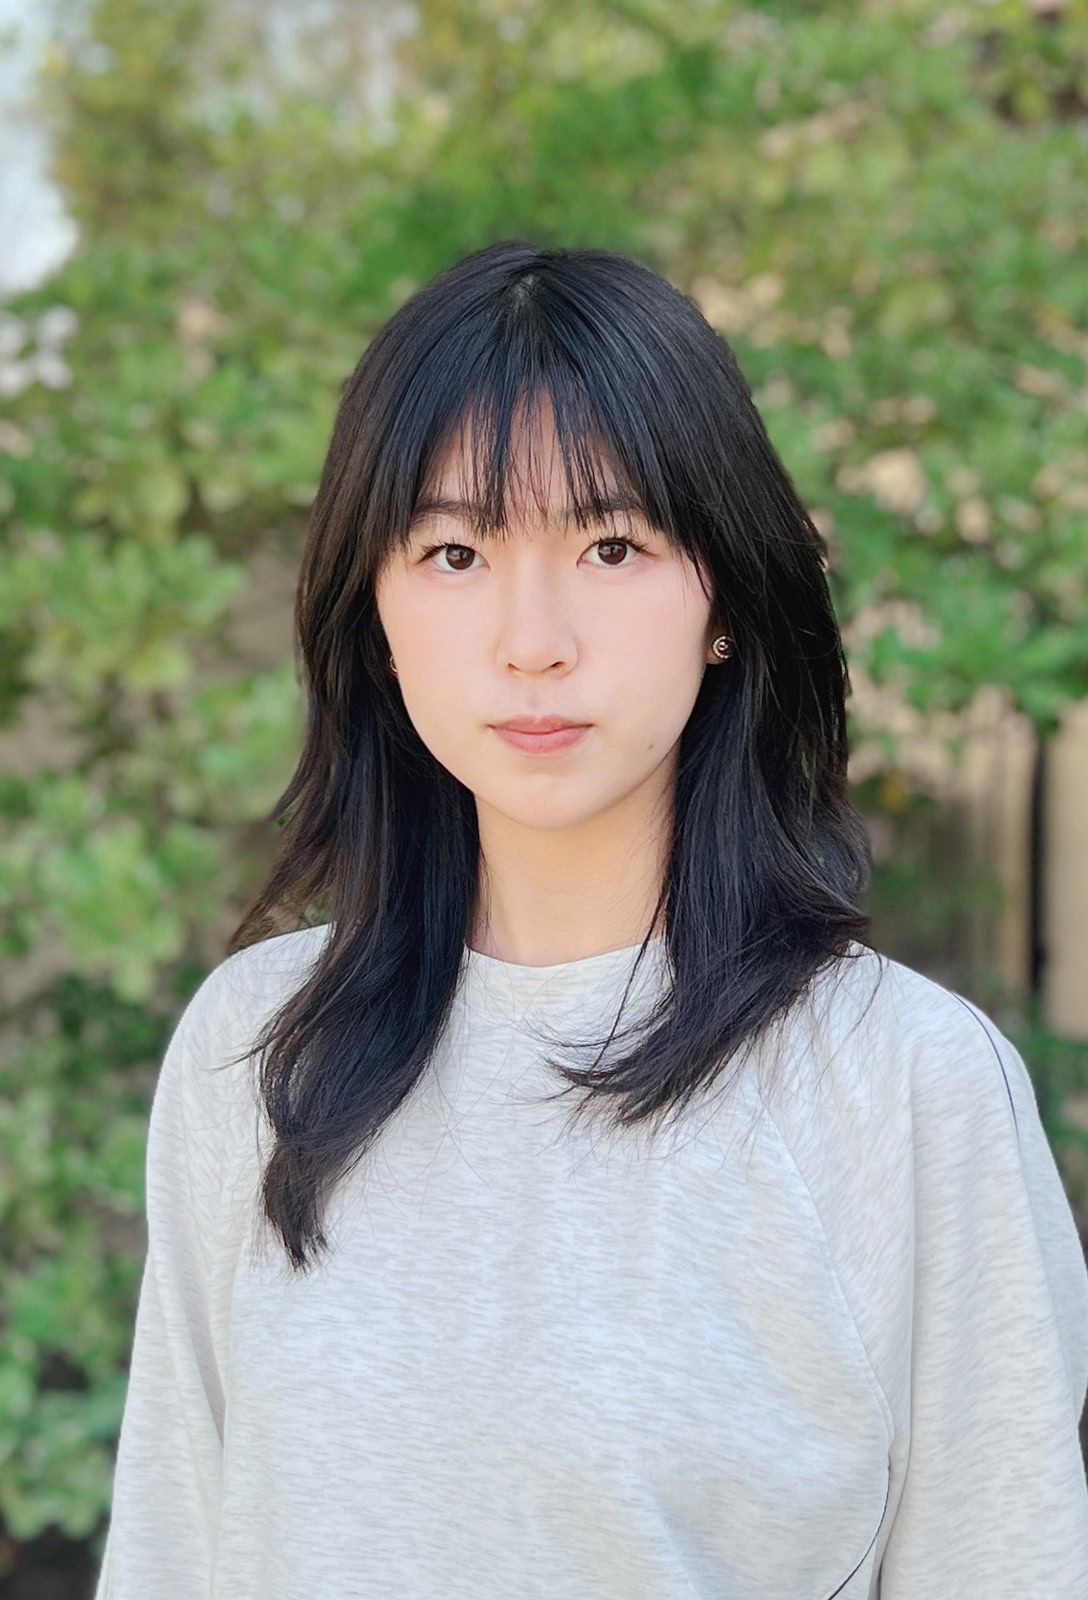
\includegraphics[width=1in,height=1.25in,clip,
    keepaspectratio]{figures/author_photo.jpeg}}]{SOPHIE ZHU}
is a student at Mira Costa High School, in Manhattan Beach, CA, USA. Her research interests include computer vision and machine learning applications in public health, with an emphasis on low-cost systems for resource-constrained environments. Her current work examines how dataset construction shapes what image classifiers learn.
\end{IEEEbiography}

\EOD
\par\vskip 0pt plus 1000fil

\end{document}
